%% LyX 2.3.5.2 created this file.  For more info, see http://www.lyx.org/.
%% Do not edit unless you really know what you are doing.
\documentclass[12pt,3p]{elsarticle}
\usepackage{mathptmx}
\renewcommand{\familydefault}{\rmdefault}
\usepackage[T1]{fontenc}
\usepackage[utf8]{inputenc}
\usepackage{color}
\usepackage{array}
\usepackage{float}
\usepackage{multirow}
\usepackage{amsmath}
\usepackage{amssymb}
\usepackage{graphicx}
\usepackage{rotfloat}
\usepackage[unicode=true,
 bookmarks=true,bookmarksnumbered=true,bookmarksopen=false,
 breaklinks=false,pdfborder={0 0 1},backref=false,colorlinks=true]
 {hyperref}

\makeatletter

%%%%%%%%%%%%%%%%%%%%%%%%%%%%%% LyX specific LaTeX commands.
%% Because html converters don't know tabularnewline
\providecommand{\tabularnewline}{\\}

%%%%%%%%%%%%%%%%%%%%%%%%%%%%%% User specified LaTeX commands.
\usepackage{bm}

\usepackage[utf8]{inputenc}
\usepackage[T1]{fontenc}


%\usepackage{endfloat}
%\usepackage{refstyle}

\usepackage{lineno}
%\modulolinenumbers[5]
%\linenumbers

%\journal{Composites Part B: Engineering}
%\journal{International Journal of Non-linear Mechanics}
\journal{Aerospace Science and Technology}

\biboptions{sort&compress}

\linespread{1.2}

%%%%%%%%%%%%%%%%%%%


%%%%%%%%%%%%%%%%%%%%

\usepackage[noabbrev,nameinlink]{cleveref}
%\crefname{figure}{figure}{figures}
%\Crefname{figure}{Figure}{Figures}
\crefname{figure}{Fig.}{Figs.}
\Crefname{figure}{Fig.}{Figs.}
%\crefname{table}{table}{tables}
%\Crefname{table}{Table}{Tables}
\crefname{table}{Table}{Tables}
\Crefname{table}{Table}{Tables}
%\crefname{equation}{eq.}{eqs.}
%\Crefname{equation}{Eq.}{Eqs.}
\crefname{equation}{Eq.}{Eqs.}
\Crefname{equation}{Eq.}{Eqs.}
\crefname{section}{Section}{Sections}
\Crefname{section}{Section}{Sections}
\crefname{appendix}{}{}

%\renewcommand\equationautorefname{\@gobble}

\AtBeginDocument{%
\let\ref\cref
}

\AtBeginDocument{%
\let\Ref\Cref
}

\usepackage{caption}
\captionsetup[table]{name={Table},labelfont={bf},labelsep={newline},textformat=period,singlelinecheck=on,justification=raggedright}
\captionsetup[figure]{name={Fig.},labelfont={bf},labelsep={period},textformat=period,singlelinecheck=on,justification=raggedright}

%\captionsetup[subtable]{name={Table},labelfont={bf},labelsep={newline},textformat=period,singlelinecheck=off,justification=raggedright}
\captionsetup[subfigure]{labelfont=bf,textfont=normalfont,singlelinecheck=on,justification=raggedright}
%%%%%%%%%%%%%%%%%%%%

%\AtBeginDocument{%
%\let\ref\autoref
%\renewcommand\equationautorefname{\@gobble}
%}

%%%%%%%%%%%%%%%%%%%

\@ifundefined{showcaptionsetup}{}{%
 \PassOptionsToPackage{caption=false}{subfig}}
\usepackage{subfig}
\makeatother

\begin{document}

\title{Geometrically nonlinear flexural analysis of multilayered composite
plate using polynomial and non-polynomial shear deformation theories}

\begin{frontmatter}{}

\author{Surendra Verma\fnref{PhD}\corref{Surendra}}

\ead{surendraverma2501@gmail.com}

\author{Babu Ranjan Thakur\fnref{PhD}\corref{Babu}}

\ead{brtjsk@iitkgp.ac.in}

\author{B. N. Singh\fnref{Prof}}

\ead{bnsingh@aero.iitkgp.ac.in}

\author{D. K. Maiti\fnref{Prof}}

\ead{dkmaiti@aero.iitkgp.ac.in}

\fntext[PhD]{Research Scholar}

\fntext[Prof]{Professor}

\cortext[Babu]{Corresponding author}

\address{Department of Aerospace Engineering, IIT Kharagpur, West Bengal,
India - 721302}
\begin{abstract}
In this paper, the geometrically nonlinear bending analysis of multilayered
composite plates is carried out through a rigorous comparative study
employing Green-Lagrange and von Kármán nonlinearity. The responses
are analyzed for various transverse loads and boundary conditions,
and emphasized the impending structural condition, which requires
the consideration of full geometric nonlinearity. The study is conducted
using a $C^{0}$ finite element plate model using third-order and
non-polynomial shear deformation theories (TSDT and NPSDT). The principle
of virtual work is utilized to formulate the weak-form of governing
equations, and discretized using nine-noded Lagrange elements with
seven degrees-of-freedom per node. The performance of the present
model has been validated by comparing present results with those available
in the literature and obtained ANSYS results. The results reveal that
the consideration of Green-Lagrange nonlinearity is essential for
plates with all sides subjected to movable simply supported boundary
conditions or with one free edge. The present study also provides
a clear idea about the utilization of TSDT and NPSDT for the anti-symmetric
and symmetric cross-ply plate, respectively, to get more accurate
solution. Further, the effect of penalty for various theories and
problems is also highlighted, and its prominent impact is asserted
for some cases. 
\end{abstract}
\begin{keyword}
Green-Lagrange nonlinearity; Higher-order shear deformation theory
(HSDT); Finite element method
\end{keyword}

\end{frontmatter}{}

\section{Introduction}

The multilayered composite structures such as laminated and sandwich
plates are being widely used in the engineering nowadays, and by virtue
of their application, they often undergo large deflection of the order
of their thickness. The range of their applications lies in aerospace,
automobile, defense, railways, shipbuilding, biomedical, polymeric
electronic, and other fields. In other words, these multilayered composite
material has almost covered every engineering sector ranging from
the deep ocean to high in the sky. The reason for this wide application
could be attributed to the high stiffness-to-weight ratio, high strength-to-weight
ratio, which are accommodated by the composite material through the
optimized ply-orientation and thickness variation of plies. Further,
the transverse loads are often prominent in these areas of application,
making it necessary to consider the shear deformation and the transverse
direction characteristic behavior. The composite plate exhibits more
transverse shear effects than the isotropic plate due to their low
transverse shear moduli relative to the in-plane Young's moduli \citep{Thakur_2020}.
Hence, for a reliable prediction of flexural characteristic of multilayered
composite plates, shear deformation need to be considered in the modeling.

Therefore, to facilitate the design and analysis process of the multilayered
composite plate, different laminated plate theories have been proposed.
First in such is the classical laminated plate theory (CLPT), which
relies on the assumption of transverse normality and neglects the
transverse shear deformation \citep{Gupta_2019}. Following that,
first-order shear deformation theory (FSDT) has been proposed, which
relaxes the transverse normality condition and accounts for constant
transverse shear deformation. However, this leads to a non-zero traction
condition at the top and bottom surfaces of the plate \citep{Sayyad_2015}.
Later, higher-order shear deformation theories (HSDTs) are developed,
which ensure traction free boundary condition at the top and bottom
surfaces along with parabolic variation of transverse stresses and
yield accurate structural analysis \citep{Abrate_2017}.

For multilayered composite plates, HSDTs with five field variables
are most popular due to the following properties: simple implementation,
cheaper computation, and reasonable accuracy compared to other HSDTs
with more than five field variables \citep{Abrate_2017}. These higher-order
shear deformation theories (HSDTs) with five field variables either
consider displacement fields of higher-order terms from Taylor's series
expansion, called polynomial shear deformation theories (PSDTs), or
consider non-polynomial function in the displacement field, called
non-polynomial shear deformation theory (NPSDT). Among PSDTs, Reddy's
third-order shear deformation (TSDT) is well noted for its accuracy
and is well diffused among the researchers. While the NPSDTs with
non-polynomial function are further classified as trigonometric ,
algebraic, hyperbolic, exponential , logarithmic, and mixed shear
deformation theories. Moreover, the list of NPSDTs is huge \citep{Sayyad_2015,Abrate_2017}.
 Recently, NPSDTs have been used for the static analysis of (advanced)
composite plate by various researchers \citep{Grover_2013,Nguyen_2016,Singh_2017,Gupta_2019,Lal_2020,Thakur_2020,Mantari_2014a,Mantari_2014b,Yarasca_2017,Mantari_2018,Monge_2018,Monge_2020}.
Among the aforementioned NPSDTs, the accuracy of inverse hyperbolic
shear deformation theory (IHSDT), developed by Grover et al. \citep{Grover_2013},
is also well noticed in the literature \citep{Grover_2013,Nguyen_2016,Gupta_2019,Thakur_2020,Thakur_2021}.
However, as per authors' knowledge, the various aspects of bending
analysis using NPSDTs (IHSDT in the present study) have not been adequately
addressed in many ways, like anti-symmetric cross-ply, penalty parameter,
etc. Hence, there is an essential need to rectify these discrepancies
in the avaiable literature for NPSDT.

Further, the laminated plates, often used as thin plates, exhibit
nonlinear behavior under large load amplitude. This nonlinearity is
mainly originated due to large displacement, because of the closeness
of yield and fracture criteria in the characteristic of laminated
composite material. In many instances, the assumption of linearity
leads to a reasonable idealization of the system behavior. Moreover,
a linear solution is obtained with considerable ease and lesser computation
than a nonlinear solution. However, in some cases, this may result
in an unrealistic approximation of the response. Over the last decades,
the large deformation analysis of the multilayered composite plates
has been the subject of interest of many investigators using analytical\textcolor{black}{{}
\citep{Shufrin_2010} or numerical }\citep{Dash_2014,Tran_2015,Phung_Van_2015,Ansari_2020,Bennaceur_2019}\textcolor{black}{{}
me}thods. Among different numerical methods, the finite element method
has been the most popular and practical numerical tool for analyzing
composite structures.

In general, the finite element method is often based on the displacement
approach, which utilizes $C^{0}$ continuous Lagrange and $C^{1}$
continuous Hermite approximations. However, the $C^{0}$ finite element
formulation is more prevalent due to ease in the implementation. Furthermore,
very few finite element packages provide support for the Hermite element.
For instance, among various open-source FE packages, i.e., code\_Aster,
GetFEM++, Deal II, Range, Elmerfem, MOOSE, libMesh, FEniCS, FEA Tool
Multiphysics, Fired ake, COMSOL(R), only GetFEM++ and FEA Tool Multiphysics
support Hermite element. Moreover, to utilize $C^{0}$ finite element
formulation in conjunction with HSDTs, penalty constraints need to
be considered to reduce the $C^{1}$ continuity of HSDTs. For instance,
the $C^{0}$ finite element approach has been considered by several
investigators \citep{Fukunaga_2001,Lal_2016,Singh_2017,Adhikari_2018,Lal_2020,Kumar_2020CL}.
However, most of aforementioned refrences have not considered the
penalty constraints \citep{Lal_2016,Singh_2017,Lal_2020,Kumar_2020CL}.
Whereas, those who have considered have not illustrated the effect
of different penalty constraints \citep{Fukunaga_2001,Adhikari_2018}.
Moreover, among these, only a few \citep{Lal_2016,Singh_2017,Kumar_2020CL}
have focused on nonlinear bending analysis using $C^{0}$ FEM.

In the context of nonlinear bending analysis of laminated plate, extensive
studies have been carried out by various investigators. However, most
of studies are limited to von Kármán nonlinearity \citep{Hari_Kishore_2011,Tsushima_2019,Javani_2019}
utilizing different modeling technique, i.e., CLPT \citep{Zaghloul_1975,Mila_inovi__2011,Ren_2018},
FSDT \citep{Shukla_2000,Liew_2004,Zhang_2005,Zhang_2006,Urthaler_2008,Rama_2018},
simplified TSDT \citep{Lim_1988,Singh_1994,Trinh_2019}, PSDTs \citep{Putcha_1986,Lim_1990,Tran_2015,Phung_Van_2015,Zhang_2015,Hirwani_2018,Vuong_2018,Ghannadpour_2020},
higher-order shear and normal deformation theory (HSNDT) \citep{Tran_2018},
Layerwise theory \citep{Cheng_1999,cetkovic2011geometrically} and
NPSDTs \citep{Dau_2006,Singh_2012,Lal_2016,Singh_2017,Kumar_2020}.
 On the other hand, very few studies have been conducted incorporating
Green-Lagrange nonlinearity \citep{Zafarmand_2019,Thakur_2021} using
FSDT \citep{Singh_1987,Le_Manh_2015}, PSDTs \citep{Sahoo_2016},
HSNDT \citep{Dash_2010,TALHA_2011,Dash_2014,Alijani_2014,Sahoo_2016,Hirwani_2018},
and Carrera Unified Formulation (CUF) \citep{Wu_2019,Pagani_2020}.
For instance, Singh and Rao \citep{Singh_1987}, using FSDT, pointed
out the importance of full Green-Lagrange nonlinearity in comparison
to von Kármán nonlinearity, for the thick laminated plates. Their
study shows that the addition of extra nonlinear term in the strain
displacement relation affects the central deflection by 13\%. Le-Manh
et al. \citep{Le_Manh_2015} studied the nonlinear behavior of composite
plate by considering large displacement, large in-plane strain, and
small rotations via isogeometric analysis associated with FSDT. The
study shows the importance of Green-Lagrange strain with small rotation
over von Kármán strain in complex boundary conditions using FSDT.
 Wu et al. \citep{Wu_2019} proposed a full geometric nonlinear plate
model using Carrera Unified Formulation (CUF) for isotropic rectangular
plates via means of Total Lagrangian approach. They have also shown
that von Kármán and Green-Lagrange results are only consistent in
loads with small magnitude for a moderately thick isotropic plate.
Note that, in the aforementioned papers on nonlinear bending analysis
of laminated composite plates, the application of Green-Lagrange nonlinearity
is limited to plates with all edges subjected to some boundary constraints.
However, in aerospace, automobile, and others, where plates are allowed
to move freely, having no geometric boundary conditions, are highly
prevalent. The only available paper in this regard is by Le-Manh et
al. \citep{Le_Manh_2015} which considers the one free edge plate
with the remaining three sides subjected to immovable boundary conditions
using FSDT in conjunction with small rotation Green-Lagrange nonlinearity.
Moreover, no paper is available which utilizes TSDT or NPSDT with
Green-Lagrange nonlinearity for nonlinear analysis despite the defused
popularity of TSDT and various developed NPSDTs for laminated plates.
Further, as per authors' best knowledge, the need of Green-Lagrange
nonlinearity over von Kármán nonlinearity in bending analysis is not
established despite of various studies have been carried out through
Green-Lagrange nonlinearity.

In comparison to the laminated plate, very few studies have been conducted
on the sandwich composite plate for nonlinear analysis \citep{Elmalich_2013,Madhukar_2013,Liang_2016,That_Hoang_2018,Katariya_2018,Rezaiee_Pajand_2019}.
     For instance, That-Hong et al. \citep{That_Hoang_2018}
formulated a four-noded quadrilateral plate element by combining cell-based
smoothed strain with TSDT for geometrically nonlinear analysis. 
Note that, in the aforementioned papers \citep{Elmalich_2013,Madhukar_2013,Liang_2016,That_Hoang_2018,Katariya_2018}
higher-order shear deformation theory, particularly TSDT, was used
for modeling the plate displacements. However, as per authors' best
knowledge, the literature on the application of NPSDT for nonlinear
bending analysis of the sandwich plate is scarcely available. 

From the concise literature reviewed above, it can be noticed that
the geometrically nonlinear behavior of laminated composite structures
has been extensively studied by different numerical methods. Among
them, FEM is the most preferred tool to study structural behavior
due to its popular and well established mathematical background. However,
most FEM studies have been limited to von Kármán's sense of nonlinearity,
while very few studies have been reported with Green-Lagrange nonlinearity.
As per authors' knowledge, despite the development of various new
non-polynomial shear deformation theories (NPSDTs) \citep{Sayyad_2015,Abrate_2017},
no literature has been reported on nonlinear static analysis using
NPSDT with full geometric nonlinearity. Thus, it is essential to conduct
a study to get a clear understanding of the efficiency of these newly
developed NPSDTs for nonlinear static analysis. Moreover, it is observed
in the literature that the accuracy of NPSDT for anti-symmetric cross-ply
is severely lacking. 

In this paper, we have illustrated the importance of Green-Lagrange
nonlinearity over von Kármán nonlinearity for nonlinear bending analysis
of multilayered composite plate through a rigorous comparison study.
For comparison, various boundary conditions such as movable and immovable
simply supported, and hinged boundary conditions with and without
rotation are considered at different load amplitudes. Further, this
same comparison is carried out for a plate with one free edge. An
energy approach is utilized to formulate the weak form of the equilibrium
equations. For kinematic modeling of the plate, both TSDT and IHSDT
in the framework of generalized higher-order shear deformation theory
(HSDT) are considered and then discretized using a nine-noded penalty
based $C^{0}$ finite element. Then, the obtained set of nonlinear
equations is incrementally solved via Newton-Raphson method. The results
reveal that the performance of IHSDT and TSDT is found to be better
in the symmetric and anti-symmetric cross-ply laminated plates, respectively.
Further, the penalty parameter has a prevailing impact on the accuracy
of the thick anti-symmetric cross-ply laminated plate and less effect
on the symmetric cross-ply laminated plate. The present study suggests
the use of Green-Lagrange nonlinearity for nonlinear bending analysis
of multilayered composite plate subjected to in-plane movable (normal)
displacement constraint for better prediction of the structural response. 

The rest of the paper is organized as follows. \ref{sec:Mathematical-formulation}
describes the mathematical formulation. In \ref{sec:Finite-element-formulation},
the set of governing equations is derived in the finite element context.
In \ref{sec:Numerical-results-and}, the accuracy of the present method
is established by comparing the obtained results with those available
in the literature and results obtained by ANSYS for thin isotropic
plates and for thin and thick laminated plates subjected to different
boundary condition with one free edge. Subsequently, parametric studies
considering various side-to-thickness ratio, number of layers, and
fiber orientation are presented for in-plane movable (normal) simply
supported boundary condition. In \ref{sec:Concluding-remarks}, a
conclusion is drawn based on this study which suggests the use of
Green-Lagrange nonlinearity for analysis when structure possesses
in-plane movable (normal) simply supported condition or free edge/s.

\section{Mathematical formulation\label{sec:Mathematical-formulation}}

A rectangular multilayered composite plate composed of $n$ elastic
orthotropic layers stacked in particular sequence $\left(\theta_{1}/\theta_{2}/\theta_{3}/\theta_{4}/\ldots/\theta_{n}\right)$
is considered. The plate dimensions are named as length $a$, width
$b$, and uniform thickness $h$. A Cartesian coordinate system, with
$x-y$ plane coinciding with middle plane of the plate, is chosen
as shown in \ref{fig:Multilayered_Composite_Plate}.
\begin{center}
\begin{figure}[H]
\centering{}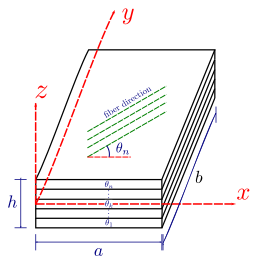
\includegraphics[width=8cm]{Plots/Laminated_Composite_Plate_AIAA_2020}\caption{\label{fig:Multilayered_Composite_Plate}Schematic diagram of multilayered
composite plate with $x-y-z$ Cartesian coordinate system}
\end{figure}
\par\end{center}

\subsection{Higher-order shear deformation theory}

Based on the characteristics of equivalent higher-order shear deformation
theory with five field variables \citep{Gupta_2019}, the assumed
displacement field can be defined in general form as follows:

\begin{equation}
\begin{gathered}u\left(x,y,z\right)=u_{0}\left(x,y\right)-z\frac{\partial w_{0}}{\partial x}+f\left(z\right)\theta_{x}\left(x,y\right)\\
v\left(x,y,z\right)=v_{0}\left(x,y\right)-z\frac{\partial w_{0}}{\partial y}+f\left(z\right)\theta_{y}\left(x,y\right)\\
w\left(x,y,z\right)=w_{0}\left(x,y\right)
\end{gathered}
\label{eq:HSDT}
\end{equation}

where, $u$, $v$, and $w$ are the displacements of arbitrary point
in $x$, $y$, $z$ directions, respectively; $u_{0}$, $v_{0}$,
and $w_{0}$ denote the midplane displacements, respectively; $\theta_{x}$
and $\theta_{y}$ represent the shear deformation of midplane normal
about $y$-axis and $x$-axis, respectively; and $f\left(z\right)$
is a thickness function. If thickness function, $f\left(z\right)$
is a polynomial or non-polynomial function of $z$, then the theory
is named as polynomial (PSDT) or non-polynomial shear deformation
theory (NPSDT), respectively. Usually, the function, $f\left(z\right)$
is such that it satisfy zero transverse shear deformation at the top
and bottom surfaces of the plate.

As pointed out in the introduction section, most displacement based
finite element models use Lagrange basis function which satisfy only
$C^{0}$ continuity of the field variables. As approximating the solution
for $C^{1}$ continuity with Hermite basis function has its own difficulty
in implementation of finite element code \citep{Serdoun_2016}. To
formulate the finite element model with HSDT (given in \ref{eq:HSDT})
using Lagrange element, an artificial field variables need to be considered
which in turn reduces the required continuity to $C^{0}$. This conversion
is compensated by penalty constraints on the strain energy \citep{Reddy_2004}
shown in following subsection. Considering the above assumption, HSDT
now contains seven field variables, $\left\{ \boldsymbol{u}\right\} $
$=$ $\{$$u_{0}$, $v_{0}$, $w_{0}$, $\phi_{x}=-\frac{\partial w_{0}}{\partial x}$,
$\phi_{y}=-\frac{\partial w_{0}}{\partial y}$, $\theta_{x}$, $\theta_{y}$$\}^{T}$
and same is expressed as:

\begin{equation}
\begin{gathered}u\left(x,y,z\right)=u_{0}\left(x,y\right)+z\phi_{x}+f\left(z\right)\theta_{x}\left(x,y\right)\\
v\left(x,y,z\right)=v_{0}\left(x,y\right)+z\phi_{y}+f\left(z\right)\theta_{y}\left(x,y\right)\\
w\left(x,y,z\right)=w_{0}\left(x,y\right)
\end{gathered}
\label{eq:New_HSDT}
\end{equation}


\subsection{Strain-displacement relation}

The state of strain, $\boldsymbol{\epsilon}$ at a point, using Green-Lagrange
strain relation, is given by following expression:

\begin{equation}
\boldsymbol{\epsilon}=\left\{ \begin{array}{c}
\frac{\partial u}{\partial x}\\
\frac{\partial v}{\partial y}\\
\frac{\partial u}{\partial y}+\frac{\partial v}{\partial x}\\
\frac{\partial v}{\partial z}+\frac{\partial w}{\partial y}\\
\frac{\partial u}{\partial z}+\frac{\partial w}{\partial x}
\end{array}\right\} +\frac{1}{2}\left\{ \begin{array}{c}
\left(\frac{\partial u}{\partial x}\right)^{2}+\left(\frac{\partial v}{\partial x}\right)^{2}+\left(\frac{\partial w}{\partial x}\right)^{2}\\
\left(\frac{\partial u}{\partial y}\right)^{2}+\left(\frac{\partial v}{\partial y}\right)^{2}+\left(\frac{\partial w}{\partial y}\right)^{2}\\
2\left(\frac{\partial u}{\partial x}\frac{\partial u}{\partial y}+\frac{\partial v}{\partial x}\frac{\partial v}{\partial y}+\frac{\partial w}{\partial x}\frac{\partial w}{\partial y}\right)\\
2\left(\frac{\partial u}{\partial y}\frac{\partial u}{\partial z}+\frac{\partial v}{\partial y}\frac{\partial v}{\partial z}+\frac{\partial w}{\partial y}\frac{\partial w}{\partial z}\right)\\
2\left(\frac{\partial u}{\partial x}\frac{\partial u}{\partial z}+\frac{\partial v}{\partial x}\frac{\partial v}{\partial z}+\frac{\partial w}{\partial x}\frac{\partial w}{\partial z}\right)
\end{array}\right\} =\boldsymbol{\epsilon_{l}}+\frac{1}{2}\boldsymbol{\epsilon_{nl}}\label{eq:TotalStrain}
\end{equation}

whereas, von Kármán strain relation is given as follows:

\begin{equation}
\boldsymbol{\epsilon}=\left\{ \begin{array}{c}
\frac{\partial u}{\partial x}\\
\frac{\partial v}{\partial y}\\
\frac{\partial u}{\partial y}+\frac{\partial v}{\partial x}\\
\frac{\partial v}{\partial z}+\frac{\partial w}{\partial y}\\
\frac{\partial u}{\partial z}+\frac{\partial w}{\partial x}
\end{array}\right\} +\frac{1}{2}\left\{ \begin{array}{c}
\left(\frac{\partial w}{\partial x}\right)^{2}\\
\left(\frac{\partial w}{\partial y}\right)^{2}\\
2\left(\frac{\partial w}{\partial x}\frac{\partial w}{\partial y}\right)\\
0\\
0
\end{array}\right\} =\boldsymbol{\epsilon_{l}}+\frac{1}{2}\boldsymbol{\epsilon_{nl}}\label{eq:TotalStrain-Von-Karman}
\end{equation}

By substituting the relation of modified displacement from \ref{eq:New_HSDT}
in \ref{eq:TotalStrain}, linear strain vector, $\boldsymbol{\epsilon}_{l}$
can be rewritten as:

\begin{equation}
\boldsymbol{\epsilon}_{l}=\left\{ \begin{array}{c}
\boldsymbol{\epsilon}_{lb}\\
\boldsymbol{\epsilon}_{ls}
\end{array}\right\} =\left\{ \begin{array}{c}
\boldsymbol{Z}_{lb}\hat{\boldsymbol{\epsilon}}_{lb}\\
\boldsymbol{Z}_{ls}\hat{\boldsymbol{\epsilon}}_{ls}
\end{array}\right\} \label{eq:LinearStrain}
\end{equation}

in which
\begin{center}
\begin{subequations}
\label{eq:GeneralizedLinearStrain}

\begin{equation}
\resizebox{0.95\textwidth}{!}{\ensuremath{\boldsymbol{\hat{\epsilon}}_{lb}=\left\{ \begin{array}{ccccccccc}
\frac{\partial u_{0}}{\partial x} & \frac{\partial v_{0}}{\partial y} & \frac{\partial u_{0}}{\partial y}+\frac{\partial v_{0}}{\partial x} & \frac{\partial\phi_{x}}{\partial x} & \frac{\partial\phi_{y}}{\partial y} & \frac{\partial\phi_{x}}{\partial y}+\frac{\partial\phi_{y}}{\partial x} & \frac{\partial\theta_{x}}{\partial x} & \frac{\partial\theta_{y}}{\partial y} & \frac{\partial\theta_{x}}{\partial y}+\frac{\partial\theta_{y}}{\partial x}\end{array}\right\} ^{T};\,\,\boldsymbol{Z}_{lb}=\left[\begin{array}{ccccccccc}
1 & 0 & 0 & z & 0 & 0 & f\left(z\right) & 0 & 0\\
0 & 1 & 0 & 0 & z & 0 & 0 & f\left(z\right) & 0\\
0 & 0 & 1 & 0 & 0 & z & 0 & 0 & f\left(z\right)
\end{array}\right]}}
\end{equation}

\begin{equation}
\boldsymbol{\hat{\epsilon}}_{ls}=\left\{ \begin{array}{cccc}
\frac{\partial w_{0}}{\partial y}+\phi_{y} & \frac{\partial w_{0}}{\partial x}+\phi_{x} & \theta_{y} & \theta_{x}\end{array}\right\} ^{T};\,\,\boldsymbol{Z}_{ls}=\left[\begin{array}{cccc}
1 & 0 & f'\left(z\right) & 0\\
0 & 1 & 0 & f'\left(z\right)
\end{array}\right]
\end{equation}
\end{subequations}
\par\end{center}

Similarly, nonlinear strain vector, $\boldsymbol{\epsilon}_{nl}$
can be reorganized as follows:

\begin{equation}
\boldsymbol{\epsilon}_{nl}=\left\{ \begin{array}{c}
\boldsymbol{\epsilon}_{nlb}\\
\boldsymbol{\epsilon}_{nls}
\end{array}\right\} =\left\{ \begin{array}{c}
\boldsymbol{Z}_{nlb}\hat{\boldsymbol{\epsilon}}_{nlb}\\
\boldsymbol{Z}_{nls}\hat{\boldsymbol{\epsilon}}_{nls}
\end{array}\right\} =\left\{ \begin{array}{c}
\boldsymbol{Z}_{nlb}\boldsymbol{A}_{b}\boldsymbol{\phi}_{b}\\
\boldsymbol{Z}_{nls}\boldsymbol{A}_{s}\boldsymbol{\phi}_{s}
\end{array}\right\} \label{eq:NonLinearStrain}
\end{equation}

in which
\begin{center}
\begin{subequations}
\label{eq:GeneralizedNonLinearStrain}

\begin{equation}
\boldsymbol{Z}_{nlb}=\resizebox{\textwidth}{!}{\ensuremath{\left[\begin{array}{cccccccccccccccccc}
1 & 0 & 0 & z & 0 & 0 & f\left(z\right) & 0 & 0 & z^{2} & 0 & 0 & zf\left(z\right) & 0 & 0 & (f\left(z\right))^{2} & 0 & 0\\
0 & 1 & 0 & 0 & z & 0 & 0 & f\left(z\right) & 0 & 0 & z^{2} & 0 & 0 & zf\left(z\right) & 0 & 0 & (f\left(z\right))^{2} & 0\\
0 & 0 & 1 & 0 & 0 & z & 0 & 0 & f\left(z\right) & 0 & 0 & z^{2} & 0 & 0 & zf\left(z\right) & 0 & 0 & (f\left(z\right))^{2}
\end{array}\right]}}\label{eq:Znlb}
\end{equation}

\begin{equation}
\boldsymbol{Z}_{nls}=\left[\begin{array}{cccccccccccc}
1 & 0 & z & 0 & f\left(z\right) & 0 & f'\left(z\right) & 0 & zf'\left(z\right) & 0 & f\left(z\right)f'\left(z\right) & 0\\
0 & 1 & 0 & z & 0 & f\left(z\right) & 0 & f'\left(z\right) & 0 & zf'\left(z\right) & 0 & f\left(z\right)f'\left(z\right)
\end{array}\right]\label{eq:Znls}
\end{equation}

\begin{equation}
\boldsymbol{\phi}_{b}=\left\{ \begin{array}{cccccccccccccc}
\frac{\partial u_{0}}{\partial x} & \frac{\partial u_{0}}{\partial y} & \frac{\partial v_{0}}{\partial x} & \frac{\partial v_{0}}{\partial y} & \frac{\partial w_{0}}{\partial x} & \frac{\partial w_{0}}{\partial y} & \frac{\partial\phi_{x}}{\partial x} & \frac{\partial\phi_{x}}{\partial y} & \frac{\partial\phi_{y}}{\partial x} & \frac{\partial\phi_{y}}{\partial y} & \frac{\partial\theta_{x}}{\partial x} & \frac{\partial\theta_{x}}{\partial y} & \frac{\partial\theta_{y}}{\partial x} & \frac{\partial\theta_{y}}{\partial y}\end{array}\right\} ^{T}\label{eq:Phib}
\end{equation}

\begin{equation}
\boldsymbol{\phi}_{s}=\left\{ \begin{array}{cccccccccccccccc}
\phi_{x} & \phi_{y} & \theta_{x} & \theta_{y} & \frac{\partial u_{0}}{\partial x} & \frac{\partial u_{0}}{\partial y} & \frac{\partial v_{0}}{\partial x} & \frac{\partial v_{0}}{\partial y} & \frac{\partial\phi_{x}}{\partial x} & \frac{\partial\phi_{x}}{\partial y} & \frac{\partial\phi_{y}}{\partial x} & \frac{\partial\phi_{y}}{\partial y} & \frac{\partial\theta_{x}}{\partial x} & \frac{\partial\theta_{x}}{\partial y} & \frac{\partial\theta_{y}}{\partial x} & \frac{\partial\theta_{y}}{\partial y}\end{array}\right\} ^{T}\label{eq:Phis}
\end{equation}
\end{subequations}
\par\end{center}

\subsection{Constitutive relation}

The constitutive relation for $k^{\text{th}}$ layer of multilayered
plate can be expressed in $x-y-z$ global coordinate system as:

\[
\left\{ \begin{array}{c}
\sigma_{xx}\\
\sigma_{yy}\\
\tau_{xy}
\end{array}\right\} =\left[\begin{array}{ccc}
\bar{Q}_{11} & \bar{Q}_{12} & \bar{Q}_{16}\\
\bar{Q}_{12} & \bar{Q}_{22} & \bar{Q}_{26}\\
\bar{Q}_{16} & \bar{Q}_{26} & \bar{Q}_{66}
\end{array}\right]\left\{ \begin{array}{c}
\epsilon_{xx}\\
\epsilon_{yy}\\
\gamma_{xy}
\end{array}\right\} \hspace{0.5cm}\text{and}\hspace{0.5cm}\left\{ \begin{array}{c}
\tau_{yz}\\
\tau_{xz}
\end{array}\right\} =\left[\begin{array}{cc}
\bar{Q}_{44} & \bar{Q}_{45}\\
\bar{Q}_{45} & \bar{Q}_{55}
\end{array}\right]\left\{ \begin{array}{c}
\gamma_{yz}\\
\gamma_{xz}
\end{array}\right\} 
\]

where $\left(\sigma_{xx},\sigma_{yy},\tau_{xy},\tau_{yz},\tau_{xz}\right)$
are the stress and $\left(\epsilon_{xx},\epsilon_{yy},\gamma_{xy},\gamma_{yz},\gamma_{xz}\right)$
are the strain components of the $k^{\text{th}}$ ply in the global
coordinates, and $\bar{Q}_{ij}$ are the transformed material constants
with local coordinates at $\theta_{k}$ angle about $z$-axis as shown
in \ref{fig:Multilayered_Composite_Plate}. The expression of $\bar{Q}_{ij}$
in terms of material constants in global coordinate system can be
found in any standard finite element textbook such as \citep{Reddy_2004}.

Consequently, the inplane stress resultant and the transverse shear
resultants are defined as:
\begin{center}
\begin{subequations}
\label{eq:StressResultant}

\begin{equation}
\left[\begin{array}{cccccc}
N_{xx} & M_{xx} & P_{xx} & Q_{xx} & R_{xx} & S_{xx}\\
N_{yy} & M_{yy} & P_{yy} & Q_{yy} & R_{yy} & S_{yy}\\
N_{xy} & M_{xy} & P_{xy} & Q_{xy} & R_{xy} & S_{xy}
\end{array}\right]=\int_{-h/2}^{h/2}\left\{ \begin{array}{c}
\sigma_{xx}\\
\sigma_{yy}\\
\tau_{xy}
\end{array}\right\} \left\{ \begin{array}{cccccc}
1 & z & f\left(z\right) & z^{2} & zf\left(z\right) & f^{2}\left(z\right)\end{array}\right\} dz\label{eq:InplaneStressResultant}
\end{equation}

\begin{equation}
\left[\begin{array}{cccccc}
N_{yz} & M_{yz} & P_{yz} & Q_{yz} & R_{yz} & S_{yz}\\
N_{xz} & M_{xz} & P_{xz} & Q_{xz} & R_{xz} & S_{xz}
\end{array}\right]=\int_{-h/2}^{h/2}\left\{ \begin{array}{c}
\tau_{yz}\\
\tau_{xz}
\end{array}\right\} \left\{ \begin{array}{cccccc}
1 & z & f\left(z\right) & f'\left(z\right) & zf'\left(z\right) & f\left(z\right)f'\left(z\right)\end{array}\right\} dz\label{eq:TransverseStressResultant}
\end{equation}
\end{subequations}
\par\end{center}

\subsection{Variational Principle}

For arbitrary space variable and admissible virtual displacement $\delta\left\{ u,v,w\right\} $,
principle of virtual work for given system, using total Lagrangian
approach, is given as:

\begin{equation}
\int_{V}\left[\delta\left\{ \boldsymbol{\epsilon}\right\} ^{T}\left\{ \boldsymbol{\sigma}\right\} +\delta\left(\frac{\partial w_{0}}{\partial x}+\phi_{x}\right)^{T}\gamma\left(\frac{\partial w_{0}}{\partial x}+\phi_{x}\right)+\delta\left(\frac{\partial w_{0}}{\partial y}+\phi_{y}\right)^{T}\gamma\left(\frac{\partial w_{0}}{\partial y}+\phi_{y}\right)\right]dV=\int_{A}\delta w^{T}PdA\label{eq:PVW}
\end{equation}

where, $\gamma$ represents the penalty parameter for artificial constraints,
and the term associated with $\gamma$ is followed from penalty function
method for constrained problem \citep{Reddy_2004,Thakur_2020,Thakur_2021}.

Here, all the kinematics and stress variables are measured with respect
to undeformed configuration (i.e., Total Lagrangian approach).

The first term in the \ref{eq:PVW} represents virtual strain energy
and is written in expanded form as:
\begin{center}
\begin{subequations}
\label{eq:VirtualStrain}

\begin{equation}
\delta U=\int_{V}\left(\delta\boldsymbol{\epsilon}\right)^{T}\boldsymbol{\sigma}dzdA=\int_{V}\left(\delta\boldsymbol{\epsilon}_{l}+\delta\boldsymbol{\epsilon}_{nl}\right)\bar{Q}\left(\boldsymbol{\epsilon}_{l}+\frac{1}{2}\boldsymbol{\epsilon}_{nl}\right)dzdA
\end{equation}

\begin{equation}
=\int_{V}\left\{ \left(\delta\hat{\boldsymbol{\epsilon}}_{l}\right)^{T}\boldsymbol{Z}_{l}^{T}\bar{Q}\boldsymbol{Z}_{l}\hat{\boldsymbol{\epsilon}}_{l}+\frac{1}{2}\left(\delta\hat{\boldsymbol{\epsilon}}_{l}\right)^{T}\boldsymbol{Z}_{l}^{T}\bar{Q}\boldsymbol{Z}_{nl}\hat{\boldsymbol{\epsilon}}_{nl}+\left(\delta\hat{\boldsymbol{\epsilon}}_{nl}\right)^{T}\boldsymbol{Z}_{nl}^{T}\bar{Q}\boldsymbol{Z}_{l}\hat{\boldsymbol{\epsilon}}_{l}+\frac{1}{2}\left(\delta\hat{\boldsymbol{\epsilon}}_{nl}\right)^{T}\boldsymbol{Z}_{nl}^{T}\bar{Q}\boldsymbol{Z}_{nl}\hat{\boldsymbol{\epsilon}}_{nl}\right\} dzdA
\end{equation}
\end{subequations}
\par\end{center}

The second and third terms in the \ref{eq:PVW} represent strain energy
due to artificial constraints, and the combined expression is

\begin{equation}
\delta U_{\gamma}=\int_{V}\gamma\left[\delta\left(\frac{\partial w_{0}}{\partial x}+\phi_{x}\right)^{T}\left(\frac{\partial w_{0}}{\partial x}+\phi_{x}\right)+\delta\left(\frac{\partial w_{0}}{\partial y}+\phi_{y}\right)^{T}\left(\frac{\partial w_{0}}{\partial y}+\phi_{y}\right)\right]dzdA\label{eq:VirtualPenaltyStrain}
\end{equation}

The last term of \ref{eq:PVW} represents virtual work done by transverse
mechanical load and is expressed as

\begin{equation}
\delta W_{ext}=\int_{A}\delta w_{0}P\left(x,y\right)|_{z=h/2}dA\label{eq:VirtualWorkDone}
\end{equation}

Here, $P\left(x,y\right)|_{z=h/2}$ represents spatially distributed
transverse load acting on the top surface $\left(z=h/2\right)$. For
simplicity, the external load is considered as non-follower load,
and it does not changes with the deformation of the plate.

\section{Finite element formulation\label{sec:Finite-element-formulation}}

In finite element method, plate domain (geometry) is need to be discretized
to form a mesh of finite elements connected through nodes. In this
study, a nine-noded isoparametric Lagrange element is considered (shown
in \ref{fig:Q9Isoparametric}).
\begin{center}
\begin{figure}[H]
\begin{centering}
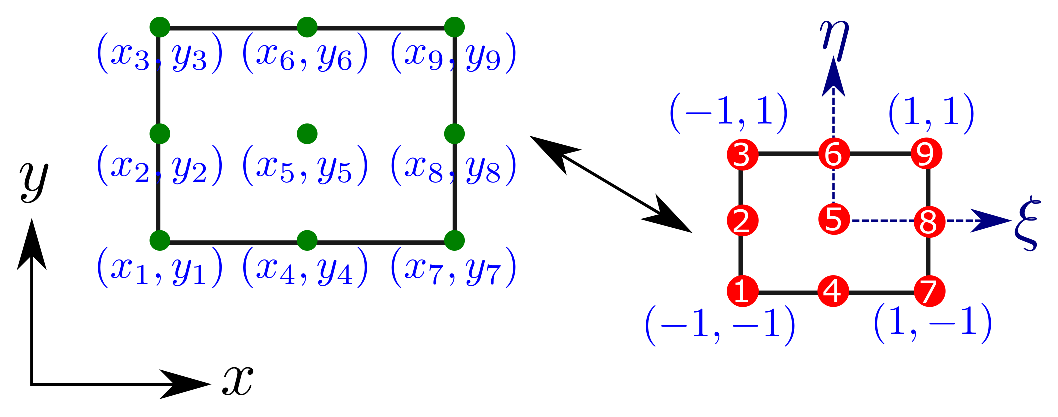
\includegraphics[scale=0.6]{Plots/Q9IsoparametricElement}\caption{\label{fig:Q9Isoparametric} Nine-noded isoparametric element}
\par\end{centering}
\end{figure}
\par\end{center}

Following the definition of shape function from geometric description,
the displacement field variables (in \ref{eq:New_HSDT}) are interpolated
at arbitrary point $(x,y)$ as:

\begin{equation}
x=\sum_{i=1}^{9}N_{i}x_{i};\,\,\,\,y=\sum_{i=1}^{9}N_{i}y_{i};\,\,\,\,\left\{ \boldsymbol{u}\right\} =\sum_{i=1}^{9}\left[I_{7}\right]N_{i}\left\{ \boldsymbol{q}_{i}\right\} \label{eq:Discretization}
\end{equation}

Here, $\left[I_{7}\right]$ denotes an identity matrix of order $7$
and $\boldsymbol{q}_{i}$ denotes vector of seven nodal displacement
field variables or degree of freedom, i.e., $\left\{ \boldsymbol{q}_{i}\right\} $$=$$\{$$u_{0i}$,
$v_{0i}$, $w_{0i}$, $\phi_{xi}$, $\phi_{yi}$, $\theta_{xi}$,
$\theta_{yi}$$\}^{T}$ corresponding to $i^{\text{th}}$ node with
$i^{\text{th}}$ shape function, $N_{i}$ .

The expressions for shape functions, corresponding to nodes shown
in \ref{fig:Q9Isoparametric}, are as follows:

\[
\begin{aligned}N_{1}= & \frac{1}{4}\xi\eta\left(\xi-1\right)\left(\eta-1\right); & N_{4}= & -\frac{1}{2}\left(\xi^{2}-1\right)\left(\eta-1\right)\eta; & N_{7}= & \frac{1}{4}\xi\left(\xi+1\right)\eta\left(\eta-1\right)\\
N_{2}= & -\frac{1}{2}\xi\left(\xi-1\right)\left(\eta^{2}-1\right); & N_{5}= & \left(\xi^{2}-1\right)\left(\eta^{2}-1\right); & N_{8}= & -\frac{1}{2}\xi\left(\xi+1\right)\left(\eta^{2}-1\right)\\
N_{3}= & \frac{1}{4}\xi\eta\left(\xi-1\right)\left(\eta+1\right); & N_{6}= & -\frac{1}{2}\left(\xi^{2}-1\right)\eta\left(\eta+1\right); & N_{9}= & \frac{1}{4}\xi\left(\xi+1\right)\eta\left(\eta+1\right)
\end{aligned}
\]

By substituting \ref{eq:Discretization} in \cref{eq:GeneralizedLinearStrain,eq:GeneralizedNonLinearStrain},
and with this generalized strain vector, $\hat{\boldsymbol{\epsilon}}$
can be rewritten in terms of strain displacement matrix, $\boldsymbol{B}$
and elemental displacement vector, $\boldsymbol{q}$. Here, for ease
in implementation of finite element formulation/code, the bending
and transverse shear partss are considered separately, which are uncoupled
in multilayered orthotropic composite; and the same is symbolically
expressed as:

\begin{equation}
\begin{gathered}\hat{\boldsymbol{\epsilon}}_{lj}=\sum_{i=1}^{9}\boldsymbol{B}_{ji}^{L}\boldsymbol{q}_{i}=\boldsymbol{B}_{j}^{L}\boldsymbol{q};\,\,\,\,\,\hat{\boldsymbol{\epsilon}}_{nlj}=\sum_{i=1}^{9}\boldsymbol{A}_{j}\boldsymbol{G}_{ji}^{NL}\boldsymbol{q}_{j}=\sum_{i=1}^{9}\boldsymbol{B}_{ji}^{NL}\boldsymbol{q}_{i}=\boldsymbol{B}_{j}^{NL}\boldsymbol{q}\\
\boldsymbol{q}=\left\{ \begin{array}{ccccc}
\boldsymbol{q}_{1}^{T} & \boldsymbol{q}_{2}^{T} & \cdots & \boldsymbol{q}_{8}^{T} & \boldsymbol{q}_{9}^{T}\end{array}\right\} ^{T}
\end{gathered}
\label{eq:StrainDisplacementMatrix}
\end{equation}

where, $j=\,\,'b'$ for bending and $j=\,\,'s'$ for transverse shear
part; while superscript $L$ represents the linear part, and superscript
$NL$ represents the nonlinear part. 

So the explicit expression of $\boldsymbol{B}_{j}^{L}$ and $\boldsymbol{B}_{j}^{NL}$
contains terms which require first Cartesian derivative of Lagrange
basis function, $\left(\frac{\partial N_{i}}{\partial x}\right)$.
Using chain-rule, first derivative of $N_{i}$ (in Cartesian coordinate)
can be calculated in terms of derivative with respect to parametric
coordinate ($\xi$ and $\eta$) by following relation:

\[
\left\{ \begin{array}{c}
\frac{\partial N_{i}}{\partial x}\\
\frac{\partial N_{i}}{\partial y}
\end{array}\right\} =\left[\begin{array}{cc}
\frac{\partial x}{\partial\xi} & \frac{\partial y}{\partial\xi}\\
\frac{\partial x}{\partial\eta} & \frac{\partial y}{\partial\eta}
\end{array}\right]^{-1}\left\{ \begin{array}{c}
\frac{\partial N_{i}}{\partial\xi}\\
\frac{\partial N_{i}}{\partial\eta}
\end{array}\right\} 
\]

Similarly, strain-displacement matrix for \ref{eq:VirtualPenaltyStrain}
can also be obtained in similar manner and virtual strain energy due
to penalty can be rewritten as:

\begin{equation}
\delta U_{\gamma}=\left(\delta\boldsymbol{q}\right)^{T}\int_{V}\left[\boldsymbol{B}_{\gamma}\right]^{T}\left[\boldsymbol{B}_{\gamma}\right]\gamma dzdA\label{eq:VirtualPenaltyStrain-1}
\end{equation}


\subsection{System of equations}

By utilizing \cref{eq:Discretization,eq:StrainDisplacementMatrix}
in \cref{eq:VirtualStrain,eq:VirtualWorkDone,eq:VirtualPenaltyStrain-1}
with followed substitution into \ref{eq:PVW} and then eliminating
the virtual displacement vector, $\left(\delta\boldsymbol{q}\right)^{T}$;
the set of equations for static analysis under distributed transverse
load is obtained as:

\begin{equation}
\left(\boldsymbol{K}+\gamma\boldsymbol{K}_{\gamma}\right)\boldsymbol{q}=\boldsymbol{F}_{P}\label{eq:StaticAnalysis}
\end{equation}

in which

\begin{subequations}
\[
\boldsymbol{K}=\int_{V}\left(\left(\boldsymbol{B}^{L}\right)^{T}\boldsymbol{Z}_{l}^{T}\bar{\boldsymbol{Q}}\boldsymbol{Z}_{l}\boldsymbol{B}^{L}+\frac{1}{2}\left(\boldsymbol{B}^{L}\right)^{T}\boldsymbol{Z}_{l}^{T}\bar{\boldsymbol{Q}}\boldsymbol{Z}_{nl}\boldsymbol{B}^{NL}+\left(\boldsymbol{B}^{NL}\right)^{T}\boldsymbol{Z}_{nl}^{T}\bar{\boldsymbol{Q}}\boldsymbol{Z}_{l}\boldsymbol{B}^{L}+\frac{1}{2}\left(\boldsymbol{B}^{NL}\right)^{T}\boldsymbol{Z}_{nl}^{T}\bar{\boldsymbol{Q}}\boldsymbol{Z}_{nl}\boldsymbol{B}^{NL}\right)dzdA
\]

\[
\boldsymbol{K}_{\gamma}=\int_{V}\left[\boldsymbol{B}_{\gamma}\right]^{T}\left[\boldsymbol{B}_{\gamma}\right]dzdA;\,\,\,\,\boldsymbol{F}_{P}=\int_{A}\left\{ \mathcal{W}\right\} P\left(x,y\right)dA
\]
\end{subequations}

where

\[
\left\{ \mathcal{W}\right\} \left\{ \boldsymbol{q}\right\} =\sum_{i=1}^{9}\left\{ \mathcal{W}_{i}\right\} \boldsymbol{q}_{i};\,\,\,\,\left\{ \mathcal{W}_{i}\right\} =\left\{ \begin{array}{ccccccc}
0 & 0 & N_{i} & 0 & 0 & 0 & 0\end{array}\right\} 
\]


\subsection{Solution procedure}

In this section, solution procedure for nonlinear algebraic equations,
\ref{eq:StaticAnalysis} is discussed. After assembling elemental
set of equation for all finite elements and imposing the suitable
boundary conditions, the nonlinear system of algebraic equations is
solved iteratively. There are several iterative approaches to solve
these nonlinear set of equations and the fundamental impetus behind
these approaches is the residual due to the assumed solution.

As present study is confined to plate structure only, subjected to
transverse load, which generally do not exhibit snap-back and snap-through
behavior. Thus, for nonlinear static analysis, Newton-Raphson iterative
method  is employed to obtain the solution for the discrete incremental
mechanical load step. For each incremental load, the incremental change
in the displacement, $\Delta\boldsymbol{q}$ can be defined for $n^{\text{th}}$
iteration:

\[
\Delta\boldsymbol{q}=\frac{\left(\boldsymbol{F}_{P}-\left(\boldsymbol{K}\left(\boldsymbol{q}_{n}\right)-\gamma\boldsymbol{K}_{\gamma}\right)\boldsymbol{q}_{n}\right)}{\boldsymbol{K}_{T}}
\]

where, $\boldsymbol{K}_{T}$ is the tangent stiffness matrix and is
defined as

\[
\boldsymbol{K}_{T}=\gamma\boldsymbol{K}_{\gamma}+\boldsymbol{K}_{L}+\boldsymbol{K}_{NL}+\boldsymbol{K}_{\sigma}
\]

Herein, $\boldsymbol{K}_{\sigma}=\int_{A}\left\{ \left(\boldsymbol{G}_{bj}^{NL}\right)^{T}\mathbb{N}_{b}\boldsymbol{G}_{bj}^{NL}+\left(\boldsymbol{G}_{sj}^{NL}\right)^{T}\mathbb{N}_{s}\boldsymbol{G}_{sj}^{NL}\right\} dA$

in which expression of $\mathbb{N}_{b}$ and $\mathbb{N}_{s}$ are
given in the \ref{sec:The-expression-of-Nb-and-Ns} and the combined
expression for $\boldsymbol{K}_{L}+\boldsymbol{K}_{NL}$ is given
by \ref{eq:TangentMatrix-1}.

\begin{equation}
\boldsymbol{K}_{L}+\boldsymbol{K}_{NL}=\int_{V}\left[\left\{ \left(\boldsymbol{B}^{L}\right)^{T}\boldsymbol{Z}_{l}^{T}+\left(\boldsymbol{B}^{NL}\right)^{T}\boldsymbol{Z}_{nl}^{T}\right\} \bar{\boldsymbol{Q}}\left\{ \boldsymbol{Z}_{l}\boldsymbol{B}^{L}+\boldsymbol{Z}_{nl}\boldsymbol{B}^{NL}\right\} \right]dzdA\label{eq:TangentMatrix-1}
\end{equation}

The process is repeated until the convergence criteria is satisfied.
Here, a relative displacement norm criteria:

\[
\frac{||\Delta\boldsymbol{q}||}{||\boldsymbol{q}||}<\beta
\]

is used with error tolerance, $\beta=10^{-2}$ or otherwise stated
in the problem.

\subsection{\textcolor{magenta}{Stress-recovery technique over the surface}}

\textcolor{magenta}{In this subsection, the stress-recovery technique
\citep{Zienkiewicz_1995,Akin_2005} used to obtain the continuous
and improved stress component over the surface is briefly discussed.
It is found in the literature that the performance of super convergent
patch recovery (SPR) is superior than its counter part, i.e., direct
interpolation and continuous least square projection (CL2P) techniques
\citep{Akin_2005}. Here, in this study, a SPR technique is applied
only to recover the inplane distribution of stresses.}

\textcolor{magenta}{In general, the inplane distribution of stresses
is smooth and continuous for bending problem as observed in 3D elasticity
solution \citep{Reddy_2004}. However, due to the consideration of
$C^{0}$ continuous Lagrange element as in the present finite element
model, only primary solution, i.e., displacement is found to be continuous
over the plate. Particularly, from the viewpoint of designer or engineer,
an accurate distribution of stresses is of more importance than the
displacement. In order to obtain smooth and continuous stresses over
the plate surface, a stress-recovery technique is needed to be used
in the post-processing step to obtain the accurate inplane distribution
of stresses. }

\textcolor{magenta}{Moreover, the through-thickness distribution of
transverse stresses, $\tau_{yz}$ and $\tau_{xz}$ predicted by present
FEM model is also found to be continuous due to HSDT \citep{Reddy_2004}.
Also, it is well established in the literature that the accurate distribution
of transverse stresses is possible through integration of 3D elasticity
equilibrium equations \citep{Reddy_2004,Tornabene_2016,Tornabene_2017}.
However, this approach requires second derivative of primary solution
which is less accurate or constant for lower finite element \citep{Auricchio1999}.
Hence, different researchers have used different techniques to obtain
the second derivative of displacement \citep{Tornabene_2016,Tornabene_2017,Daniel_2020}.
Further, the transverse stresses obtained through the constitutive
relation employing HSDT gives reasonably good idea about the through-thickness
variation of transverse stresses. Hence, for present study, no recovery
technique is used in thickness direction, and transverse stresses
are obtained through the constitutive relation for both von Kármán
and Green-Lagrange non-linearity. It is shown in the \ref{sec:Numerical-results-and}
that the use of constitutive approach for transverse stresses is limited
to von Kármán non-linearity only and is not useful for Green-Lagrange
nonlinearity, and the use of equilibrium approach in the thickness
direction is suggested, as done in references \citep{Tornabene_2016,Tornabene_2017,Daniel_2020}.}

\textcolor{magenta}{In SPR technique \citep{Akin_2005}, the improved
stress components, $\sigma^{*}$ is obtained by taking a least square
projection of the computed stress, $\sigma$ at sampling (Gauss-Legendre)
points over a patch. Here, a patch is defined as group of elements
with vertex node at its center. A patch can contain three or more
elements and can be classified as interior or boundary patch accordingly
as shown in \cref{fig:Interior-and-boundary-patches,fig:Four-element-patch}. }
\begin{center}
\textcolor{magenta}{}
\begin{figure}[H]
\begin{centering}
\textcolor{magenta}{}\subfloat[Interior and boundary patches\label{fig:Interior-and-boundary-patches}]{\centering{}\textcolor{magenta}{\includegraphics[scale=0.5]{\string"All_Images/Classification of Patch\string".pdf}}}
\par\end{centering}
\centering{}\textcolor{magenta}{}\subfloat[Four-element patch\label{fig:Four-element-patch}]{\centering{}\textcolor{magenta}{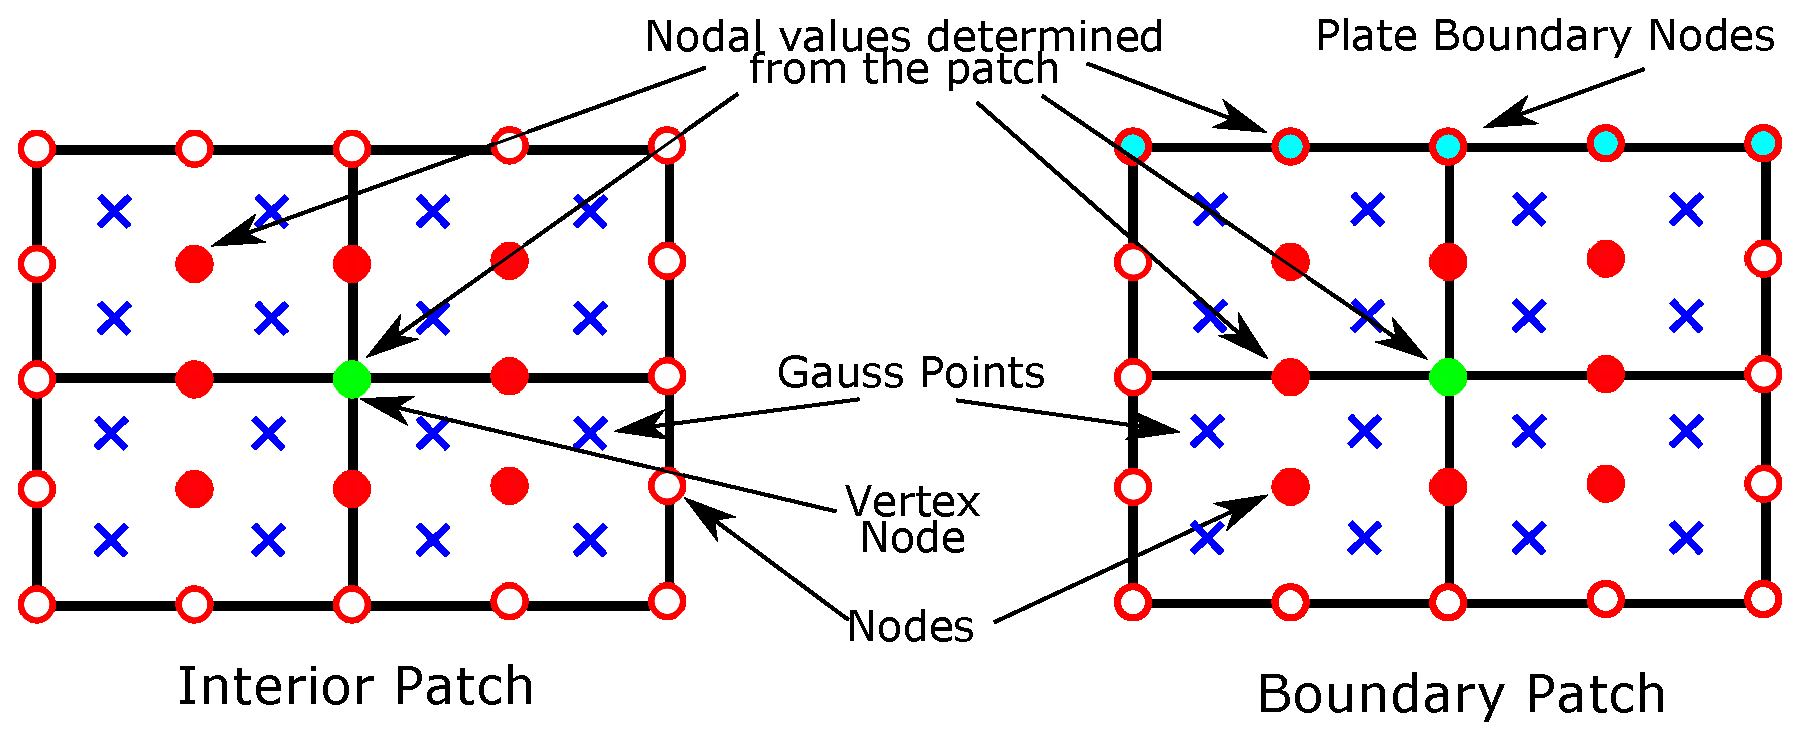
\includegraphics[scale=0.45]{All_Images/Patch}}}\textcolor{magenta}{\caption{SPR patch for Q9 Lagrange element}
}
\end{figure}
\par\end{center}

\textcolor{magenta}{In order to obtain the continuous improved stresses
over the patch for each stress component, the improved stress field,
$\sigma^{*}$ is assumed to be a form of polynomial expansion. In
present study, the polynomial expansion written in \ref{eq:Polynomial_Expansion}
is considered for modeling.
\begin{equation}
\sigma^{*}=P_{0}+\bar{x}P_{1}+\bar{y}P_{2}+\bar{x}\bar{y}P_{3}+\bar{x}^{2}P_{4}+\bar{y}^{2}P_{5}+\bar{x}^{2}\bar{y}P_{6}+\bar{x}\bar{y}^{2}P_{7}+\bar{x}^{2}\bar{y}^{2}P_{8}\label{eq:Polynomial_Expansion}
\end{equation}
}

\textcolor{magenta}{or 
\[
\sigma^{*}=\mathcal{M}_{i}P_{i}=\boldsymbol{\mathcal{M}}\boldsymbol{P}
\]
}

\textcolor{magenta}{where, $P_{i}$ is the unknown coefficient to
be determined for each stress component in a patch with $\bar{x}=x_{sp}-x_{v}$
and $\bar{y}=y_{sp}-y_{v}$. Here, $x_{sp}$ and $x_{v}$ represent
the x-coordinate of sampling and vertex points, respectively. }

\textcolor{magenta}{It is to be noted that any suitable polynomial
expansion can be considered according to the number of sampling points
and number of unknown coefficients taken in a single patch. As stated
above, the unknown expansion coefficients are determined by making
it fit the calculated stresses at the set of sampling points inside
the patch in a least square manner which is defined as}

\textcolor{magenta}{
\[
\mathcal{F}=\frac{1}{2}\left(\sigma^{*}-\sigma\right)^{T}\left(\sigma^{*}-\sigma\right)d\Omega_{p}
\]
}

\textcolor{magenta}{
\[
\int_{\Omega_{p}}\frac{\partial\mathcal{F}}{\partial P_{i}}=\int_{\Omega_{p}}\left(\frac{\partial\sigma^{*}}{\partial P_{i}}\right)^{T}\left(\sigma^{*}-\sigma\right)d\Omega_{p}=0
\]
}

\textcolor{magenta}{or}

\textcolor{magenta}{
\[
\int_{\Omega_{p}}\boldsymbol{\mathcal{M}}^{T}\boldsymbol{\mathcal{M}}d\Omega_{p}\boldsymbol{P}=\int_{\Omega_{p}}\boldsymbol{\mathcal{M}}^{T}\sigma d\Omega_{p}\text{ or }\boldsymbol{A}\boldsymbol{P}=\boldsymbol{B}
\]
}

\textcolor{magenta}{in which,}

\textcolor{magenta}{
\[
\boldsymbol{A}=\int_{\Omega_{p}}\boldsymbol{\mathcal{M}}^{T}\boldsymbol{\mathcal{M}}d\Omega_{p}\text{ and }\boldsymbol{B}=\int_{\Omega_{p}}\boldsymbol{\mathcal{M}}^{T}\sigma d\Omega_{p}
\]
}

\textcolor{magenta}{Here, the symbol $\Omega_{p}$ represents the
patch domain. After solving for the unknown coefficient, $P_{i}$
for each stress component, the required stress value at selected nodes
(see \ref{fig:Four-element-patch}) can be obtained using \ref{eq:Polynomial_Expansion}.
In this SPR approach, some nodes can have multiple values due to the
overlapping of patches as depicted in \ref{fig:Overlapping-of-patches}.
Hence, a simple averaging is needed to reach a unique stress value
over the surface.}
\begin{center}
\textcolor{magenta}{}
\begin{figure}[H]
\begin{centering}
\textcolor{magenta}{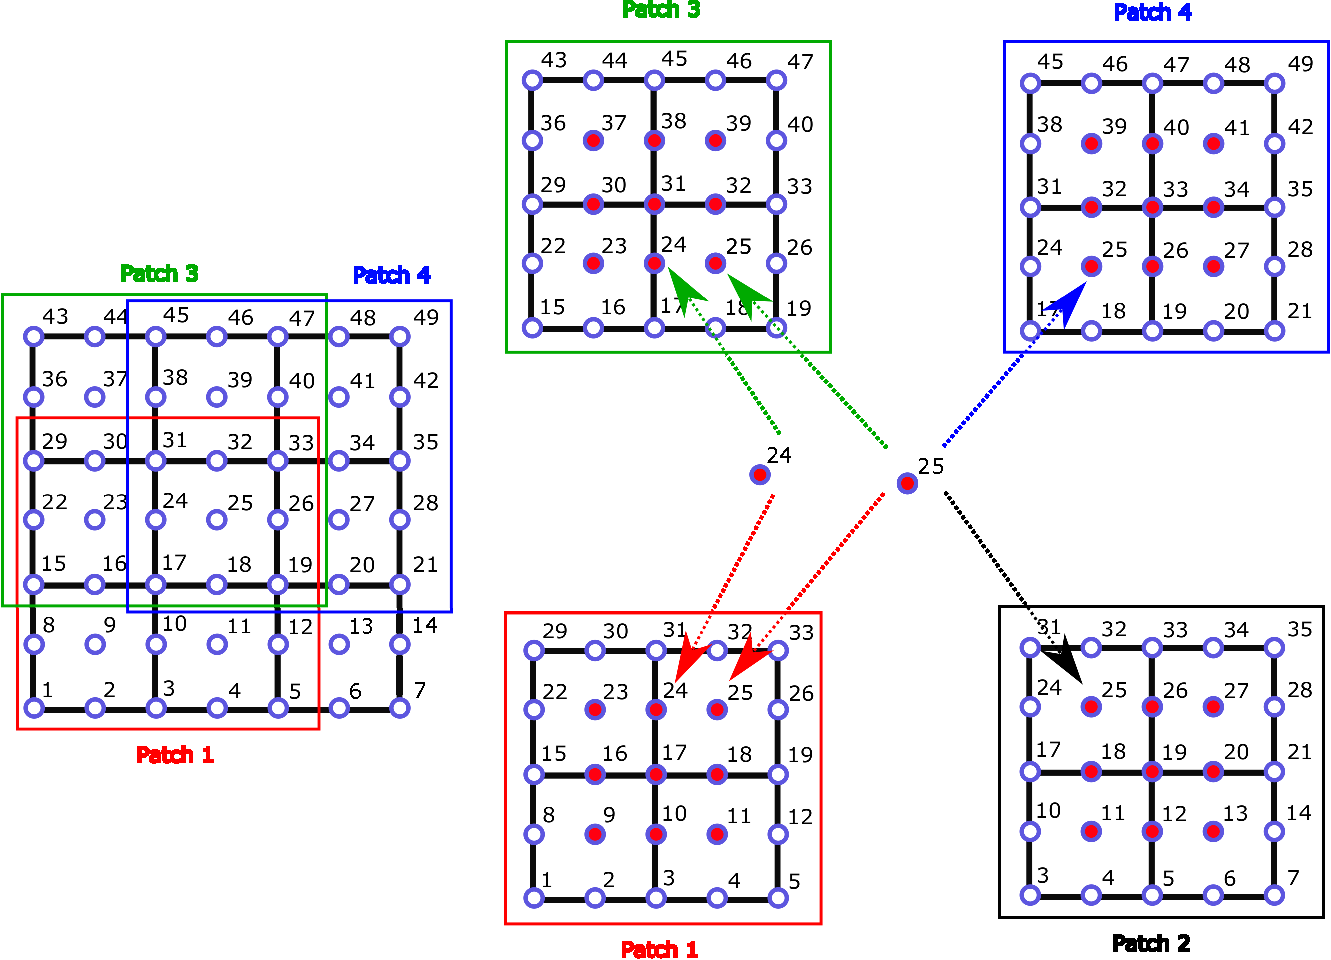
\includegraphics[scale=0.6,angle=-90]{All_Images/Assembly}\caption{Overlapping of patches\label{fig:Overlapping-of-patches}}
}
\par\end{centering}
\end{figure}
\par\end{center}

\section{Numerical results and discussions\label{sec:Numerical-results-and}}

In this section, the accuracy and efficacy of the present $C^{0}$
finite element formulation are assessed through several nonlinear
bending examples along with the effect of penalty constraints. Also,
numerical results obtained using present formulation for PSDT (specifically
TSDT), $f\left(z\right)=z-4z^{3}/3h^{2}$ \citep{Tran_2015,Reddy_2004}
and NPSDT (specifically IHSDT), $f\left(z\right)=sinh^{-1}\left(3z/h\right)-6z/h\sqrt{13}$
\citep{Grover_2013} are studied comparatively. Both present solutions
are further compared with obtained ANSYS solutions and other analytical,
experimental, and numerical solutions from the literature. The present
NPSDT, i.e., IHSDT is selected based on its analytical and numerical
performance over other theories shown in the references \citep{Grover_2013,Nguyen_2016,Gupta_2019,Thakur_2020,Thakur_2021}.


\subsection{Material properties\label{subsec:Material-properties}}

The following sets of material properties are used in subsequent section:
\begin{itemize}
\item Material-I: \citep{Le_Manh_2015}

$E_{1}/E_{2}=25$, $G_{12}/E_{2}=G_{13}/E_{2}=0.5$, $G_{23}/E_{2}=0.2$,
$\nu_{12}=0.25$
\item Material-II: \citep{Reddy_2004}

$E_{1}/E_{2}=40\text{ or variable}$, $G_{12}/E_{2}=G_{13}/E_{2}=0.6$,
$G_{23}/E_{2}=0.5$, $\nu_{12}=0.25$
\item Material-III: \citep{Zaghloul_1975,Tran_2015}

$E_{1}=3\times10^{6}\,\text{psi}\,(20.684\,\text{GPa})$, $E_{2}=1.28\times10^{6}\,\text{psi}\,(8.825\,\text{GPa})$,

$G_{12}=G_{13}=G_{23}=0.37\times10^{6}\,\text{psi}\,(2.551\,\text{GPa})$,
$\nu_{12}=0.32$
\item Material-IV: \citep{Zaghloul_1975,Tran_2015}

$E_{1}=1.8282\times10^{6}\,\text{psi}\,(12.604\,\text{GPa})$, $E_{2}=1.8315\times10^{6}\,\text{psi}\,(12.627\,\text{GPa})$,

$G_{12}=G_{13}=G_{23}=3.125\times10^{5}\,\text{psi}\,(2.155\,\text{GPa})$,
$\nu_{12}=0.2395$
\item Material-V: \citep{Ganapathi_2004,Madhukar_2013}

Facesheet: $E_{1}=139\,\text{GPa}$, $E_{2}=9.86\,\text{GPa}$, $G_{12}=G_{13}=G_{23}=5.24\,\text{GPa}$,
$\nu_{12}=0.3$

Core: $E_{1}=E_{2}=0.09\,\text{GPa}$, $G_{12}=G_{13}=G_{23}=0.032\,\text{GPa}$,
$\nu_{12}=0.45$
\end{itemize}

\subsection{Boundary conditions}

As the present formulation is based on displacement approach with
$C^{0}$ continuity, so it is required to satisfy only kinematics
boundary conditions , i.e., $($$u_{0}$, $v_{0}$, $w_{0}$, $\phi_{x}$,
$\phi_{y}$, $\theta_{x}$, $\theta_{y}$$)$. The different types
of boundary conditions, most commonly encounter in practice, are considered
for present study of full geometrically nonlinear analysis of laminated
and sandwich composite plates.
\begin{itemize}
\item Simply supported
\begin{enumerate}
\item For cross-ply \citep{Dash_2010}

SSSS1 : $u_{0}=w_{0}=\theta_{x}=\phi_{x}=0$ at $y=0,b$ and $v_{0}=w_{0}=\theta_{y}=\phi_{y}=0$
at $x=0,a$
\item For angle-ply \citep{Dash_2010}

SSSS2 : $v_{0}=w_{0}=\theta_{x}=\phi_{x}=0$ at $y=0,b$ and $u_{0}=w_{0}=\theta_{y}=\phi_{y}=0$
at $x=0,a$
\item Immovable hard (Hinged) \citep{Tran_2015}

SSSS3 : $u_{0}=v_{0}=w_{0}=\theta_{x}=\phi_{x}=0$ at $y=0,b$ and
$u_{0}=v_{0}=w_{0}=\theta_{y}=\phi_{y}=0$ at $x=0,a$
\item Immovable soft \citep{Tran_2015}

SSSS4 : $u_{0}=v_{0}=w_{0}=0$ at $y=0,b$ and $x=0,a$
\end{enumerate}
\item Clamped \citep{Dash_2010}

CCCC : $u_{0}=v_{0}=w_{0}=\theta_{x}=\theta_{y}=\phi_{x}=\phi_{y}=0$
at $y=0,b$ and $x=0,a$
\item SSFSX

S at $y=0$, S at $x=b$, no condition at $y=b$, S at $x=0$

Here, '$X$' signifies the type of simply supported, i.e., 1, 2, 3,
or 4.
\end{itemize}

\subsection{Numerical results and discussions}

In all the following examples, unless specified otherwise, all layers
are assumed to be equal in thickness, and all the present solutions
are obtained at $12\times12$ mesh discretization. \textcolor{magenta}{For
the post-processing of stresses, the superconvergent patch recovery
technique with $2\times2$ Legendre-Gauss sampling is used. }

\noindent\begin{minipage}[t]{1\columnwidth}%
\textbf{Linear analysis}%
\end{minipage}

In this part, the linear analysis has been carried out to validate
the present formulation before going for the detailed nonlinear analysis.
Moreover, to investigate the accuracy in a more authentic way, Navier
type closed form solutions (CFSs) using IHSDT have been obtained,
as there is an unavailability of the closed form solutions for some
cases. These closed form solutions are then used to assess the accuracy
of the FEM-IHSDT solution and to calibrate the value of the penalty
parameter, $\gamma$. The mathematical formulation for the Navier
type closed form solutions is shown in the \ref{sec:Navier-solution}. 

\subsubsection{Simply supported symmetric cross-ply square laminated plate under
SSL }

In order to validate the present formulation, a simply supported $\left(SSSS1\right)$
four layered $\left(0^{0}/90^{0}/90^{0}/0^{0}\right)$ square composite
plate under sinusoidal distributed load (SSL), $P=P_{0}sin\left(\pi x/a\right)sin\left(\pi y/b\right)$
is considered for investigation. The plate is made of $Material-I$
(given in \ref{subsec:Material-properties}).  The normalized deflection
and stresses computed by present FEM formulation are presented in
\ref{tab:SSSS1_SSL_0_90_90_0} for different penalty parameter, $\gamma$.
The normalized quantities used for comparison are:

\[
\begin{aligned}\bar{w}= & w_{0}\left(\frac{a}{2},\frac{b}{2}\right)\left(\frac{100E_{2}h^{3}}{a^{4}P_{0}}\right) & \bar{\sigma}_{xx}= & \sigma_{xx}\left(\frac{a}{2},\frac{b}{2},\frac{h}{2}\right)\left(\frac{h^{2}}{b^{2}P_{0}}\right)\\
\bar{\sigma}_{yy}= & \sigma_{yy}\left(\frac{a}{2},\frac{b}{2},\frac{h}{4}\right)\left(\frac{h^{2}}{b^{2}P_{0}}\right) & \bar{\tau}_{xy}= & \tau_{xy}\left(0,0,\frac{h}{2}\right)\left(\frac{h^{2}}{b^{2}P_{0}}\right)\\
\bar{\tau}_{yz}= & \tau_{yz}\left(\frac{a}{2},0,0\right)\left(\frac{h}{bP_{0}}\right) & \bar{\sigma}_{yy}= & \tau_{xz}\left(0,\frac{b}{2},0\right)\left(\frac{h}{bP_{0}}\right)
\end{aligned}
\]

It can be observed from the \ref{tab:SSSS1_SSL_0_90_90_0} that the
present solutions (for both TSDT and IHSDT using $\gamma=10^{7}$)
are found to be in good agreement with their respective Navier type
closed form solutions (CFSs). The results also reveal that the effect
of the penalty parameter is not much significant for the deflection
characterstic of a symmetric cross-ply laminated plate. The relative
change occurs in the deflection and stresses values without penalty
constraints ($\gamma=0$) is about $0.17\%$ and $3.7\%$, respectively
for IHSDT, and $0.45\%$ and $5.7\%$, respectively for TSDT with
respect to solutions using $\gamma=10^{7}$. Particularly, IHSDT yields
better solutions than TSDT at low span-to-thickness ratio ($a/h=4)$
as it is more close to 3D elasticity solution \citep{Reddy_2004}.
 
\begin{center}
\begin{table}[H]
\caption{\label{tab:SSSS1_SSL_0_90_90_0} Normalized deflection and normalized
stresses of simply supported $\left(SSSS1\right)$ four layered $\left(0^{0}/90^{0}/90^{0}/0^{0}\right)$
square laminated plate under sinusoidal distributed load (SSL)}

\centering{}%
\begin{tabular}{lllllllll}
\hline 
\multirow{2}{*}{$a/h$} & Source / & $\gamma$ & $\bar{w}$ & $\bar{\sigma}_{xx}$ & $\bar{\sigma}_{yy}$ & $\bar{\tau}_{xy}$ & $\bar{\tau}_{yz}$ & $\bar{\tau}_{xz}$\tabularnewline
 & Model & Penalty & $\left(\frac{a}{2},\frac{b}{2},0\right)$ & $\left(\frac{a}{2},\frac{b}{2},\frac{h}{2}\right)$ & $\left(\frac{a}{2},\frac{b}{2},\frac{h}{4}\right)$ & $\left(0,0,\frac{h}{2}\right)$ & $\left(\frac{a}{2},0,0\right)$ & $\left(0,\frac{b}{2},0\right)$\tabularnewline
\hline 
4 & 3D Elasticity \citep{Reddy_2004} &  & 1.9540 & 0.7200 & 0.6630 & 0.0467 & 0.2920 & 0.2190\tabularnewline
 & CFS-IHSDT \citep{Grover_2013} & - & 1.9257 & 0.7240 & 0.6396 & 0.0473 & 0.2699 & 0.2505\tabularnewline
 & CFS-TSDT \citep{Reddy_2004} & - & 1.8940 & 0.6650 & 0.6320 & 0.0440 & 0.2390 & 0.2060\tabularnewline
 & FEM-IHSDT$^{\dagger}$ & $10^{7}$ & 1.9257 & 0.7254 & 0.6390 & 0.0473 & 0.2699 & 0.2504\tabularnewline
 & FEM-TSDT$^{\dagger}$ & $10^{7}$ & 1.8937 & 0.6651 & 0.6322 & 0.0440 & 0.2390 & 0.2064\tabularnewline
 & FEM-IHSDT$^{\dagger}$ & $10^{4}$ & 1.9258 & 0.7255 & 0.6390 & 0.0473 & 0.2700 & 0.2505\tabularnewline
 & FEM-TSDT$^{\dagger}$ & $10^{4}$ & 1.8937 & 0.6651 & 0.6322 & 0.0441 & 0.2390 & 0.2065\tabularnewline
 & FEM-IHSDT$^{\dagger}$ & $0$ & 1.9290 & 0.6994 & 0.6400 & 0.0468 & 0.2706 & 0.2445\tabularnewline
 & (relative change) &  & (0.17\%) & (3.7\%) & (0.15\%) & (1\%) & (0.25\%) & (2.41\%)\tabularnewline
 & FEM-TSDT$^{\dagger}$ & $0$ & 1.9023 & 0.7057 & 0.6309 & 0.0461 & 0.2460 & 0.2138\tabularnewline
 & (relative change) &  & (0.45\%) & (5.7\%) & (0.2\%) & (4.5\%) & (2.8\%) & (3.46\%)\tabularnewline
 &  &  &  &  &  &  &  & \tabularnewline
100 & 3D-Elasticity \citep{Reddy_2004} &  & 0.4380 & 0.5390 & 0.2760 & 0.0216 & 0.1410 & 0.3370\tabularnewline
 & CFS-IHSDT \citep{Grover_2013} & - & 0.4344 & 0.5385 & 0.2710 & 0.0213 & 0.1269 & 0.3643\tabularnewline
 & CFS-TSDT \citep{Reddy_2004} & - & 0.4340 & 0.5390 & 0.2710 & 0.0213 & 0.1120 & 0.2900\tabularnewline
 & FEM-IHSDT$^{\dagger}$ & $10^{7}$ & 0.4344 & 0.5387 & 0.2709 & 0.0213 & 0.1271 & 0.3643\tabularnewline
 & FEM-TSDT$^{\dagger}$ & $10^{7}$ & 0.4343 & 0.5387 & 0.2708 & 0.0213 & 0.1117 & 0.2898\tabularnewline
 & FEM-IHSDT$^{\dagger}$ & $10^{4}$ & 0.4345 & 0.5388 & 0.2709 & 0.0213 & 0.1271 & 0.3644\tabularnewline
 & FEM-TSDT$^{\dagger}$ & $10^{4}$ & 0.4343 & 0.5387 & 0.2708 & 0.0213 & 0.1117 & 0.2899\tabularnewline
 & FEM-IHSDT$^{\dagger}$ & $0$ & 0.4345 & 0.5389 & 0.2709 & 0.0213 & 0.1278 & 0.3724\tabularnewline
 & FEM-TSDT$^{\dagger}$ & $0$ & 0.4344 & 0.5388 & 0.2708 & 0.0213 & 0.1153 & 0.3156\tabularnewline
\hline 
\multicolumn{9}{l}{$^{\dagger}$: present results using $C^{0}$ finite element approach;
CFS stands for closed form solution}\tabularnewline
\end{tabular}
\end{table}
\par\end{center}

\subsubsection{Simply supported anti-symmetric cross-ply square laminated plate
under SSL }

To the best of authors' knowledge, most of the studies available in
the literature deal with the symmetric cross-ply laminated plate,
although anti-symmetric cross-ply laminated plates are also important
and possess important application. Therefore, to get a clear understanding
of the accuracy of the present model, a comparison study has been
carried out for anti-symmetric cross-ply laminated plate. 

In this example, two $\left(0^{0}/90^{0}\right)$ and six $\left(0^{0}/90^{0}/0^{0}/90^{0}/0^{0}/90^{0}\right)$
layered anti-symmetric cross-ply laminated plates under $SSSS1$ boundary
condition, subjected to sinusoidal distributed load (SSL), $P=P_{0}sin\left(\pi x/a\right)sin\left(\pi y/b\right)$,
are considered for investigation. The plate is made of $Material-I$
(listed in \ref{subsec:Material-properties}). In \ref{tab:SSSS1_SSL_0_90_n},
present FEM solutions along with Navier type closed form solutions
(CFSs) of TSDT and IHSDT are tabulated for the given plates with different
$a/h$ ratio. It is observed from the \ref{tab:SSSS1_SSL_0_90_n}
that the effect of penalty parameter $\left(\gamma=0\right)$ is substantial
for thick $\left(a/h=4\right)$ anti-symmetric cross-ply plate, i.e.,
$5.95\%$ relative change in the deflection value with respect to
$\gamma=10^{7}$. The reason for this discrepancy can be attributed
to the presence of extensional-bending coupling in the material stiffness
matrix. Also, it is ascertained that as the number of layers increases
the importance of penalty constraints decreases due to the vanishing
of extensional-bending coupling. Hence, it is important to consider
the penalty constraint in the formulation for the anti-symmetric cross-ply
plate. In contrast to the previous example here, TSDT yields higher
and more accurate results than IHSDT as the TSDT solutions are more
close to the 3D elasticity solution of Zenkour \citep{Zenkour_2007}
which emphasize the usage of TSDT for the anti-symmetric cross-ply
plate to get the more accurate solution. 
\begin{center}
\begin{table}[H]
\begin{centering}
\caption{\label{tab:SSSS1_SSL_0_90_n} Effect of penalty parameter, $\gamma$
on normalized deflection, $\bar{w}=w_{0}\left(\frac{a}{2},\frac{b}{2}\right)\left(\frac{100E_{2}h^{3}}{a^{4}P_{0}}\right)$
of simply supported $\left(SSSS1\right)$ anti-symmetric cross-ply
$\left(0^{0}/90^{0}\right)_{n}$ square laminated plate under sinusoidal
distributed load (SSL)}
\par\end{centering}
\centering{}%
\begin{tabular}{lllllllll}
\hline 
\multirow{2}{*}{Layers} & Source / & $\gamma$ & \multicolumn{6}{l}{$a/h$}\tabularnewline
\cline{4-9} \cline{5-9} \cline{6-9} \cline{7-9} \cline{8-9} \cline{9-9} 
 & Model & Penalty & \textsf{4} & \textsf{5} & \textsf{10} & \textsf{20} & \textsf{50} & \textsf{100}\tabularnewline
\hline 
2 $\left(n=1\right)$ & CFS-IHSDT\textsf{$^{*}$} & - & 1.8898 & 1.6009 & 1.2009 & 1.0981 & 1.0691 & 1.0650\tabularnewline
 & CFS-TSDT \citep{Reddy_2004} & - & 1.9985 & 1.6670 & 1.2161 & 1.1018 & 1.0697 & 1.0651\tabularnewline
 & FEM-IHSDT$^{\dagger}$ & $10^{7}$ & 1.8898 & 1.6009 & 1.2009 & 1.0981 & 1.0691 & 1.0649\tabularnewline
 & FEM-TSDT$^{\dagger}$ & $10^{7}$ & 1.9985 & 1.6670 & 1.2161 & 1.1018 & 1.0697 & 1.0651\tabularnewline
 & FEM-IHSDT$^{\dagger}$ & $10^{4}$ & 1.8898 & 1.6009 & 1.2009 & 1.0981 & 1.0691 & 1.0650\tabularnewline
 & FEM-TSDT$^{\dagger}$ & $10^{4}$ & 1.9986 & 1.6670 & 1.2161 & 1.1018 & 1.0697 & 1.0651\tabularnewline
 & FEM-IHSDT$^{\dagger}$ & $0$ & 2.0094 & 1.6704 & 1.2159 & 1.1017 & 1.0697 & 1.0651\tabularnewline
 & (relative change) &  & (5.95\%) & (4.16\%) & (1.23\%) & (0.32\%) & (0.05\%) & (0.01\%)\tabularnewline
 & FEM-TSDT$^{\dagger}$ & $0$ & 2.0318 & 1.6852 & 1.2197 & 1.1.027 & 1.0698 & 1.0651\tabularnewline
 & (relative change) &  & (1.63\%) & (1\%) & (0.3\%) & (0.08\%) & (0.01\%) & (0\%)\tabularnewline
 &  &  &  &  &  &  &  & \tabularnewline
4 $\left(n=2\right)$ & 3D-Elasticity \citep{Zenkour_2007} & - & 1.9581 & - & 0.7624 & 0.5716 & 0.5170 & 0.5092\tabularnewline
 & CFS-IHSDT$^{*}$ & - & 1.5909 & 1.2116 & 0.6866 & 0.5518 & 0.5137 & 0.5083\tabularnewline
 & CFS-TSDT$^{*}$ & - & 1.6093 & 1.2184 & 0.6865 & 0.5517 & 0.5137 & 0.5083\tabularnewline
 &  &  &  &  &  &  &  & \tabularnewline
6 $\left(n=3\right)$ & CFS-IHSDT\textsf{$^{*}$} & - & 1.4932 & 1.1346 & 0.6344 & 0.5052 & 0.4687 & 0.4634\tabularnewline
 & CFS-TSDT \citep{Reddy_2004} & - & 1.5411 & 1.1590 & 0.6382 & 0.5060 & 0.4688 & 0.4635\tabularnewline
 & FEM-IHSDT$^{\dagger}$ & $10^{7}$ & 1.4932 & 1.1346 & 0.6344 & 0.5052 & 0.4687 & 0.4634\tabularnewline
 & FEM-TSDT$^{\dagger}$ & $10^{7}$ & 1.5411 & 1.1590 & 0.6382 & 0.5060 & 0.4688 & 0.4635\tabularnewline
 & FEM-IHSDT$^{\dagger}$ & $10^{4}$ & 1.4932 & 1.1346 & 0.6344 & 0.5052 & 0.4687 & 0.4634\tabularnewline
 & FEM-TSDT$^{\dagger}$ & $10^{4}$ & 1.5411 & 1.1590 & 0.6382 & 0.5060 & 0.4688 & 0.4635\tabularnewline
 & FEM-IHSDT$^{\dagger}$ & $0$ & 1.5277 & 1.1509 & 0.6367 & 0.5057 & 0.4688 & 0.4635\tabularnewline
 & (relative change) &  & (2.25\%) & (1.41\%) & (0.36\%) & (0.09\%) & (0.02\%) & (0.01\%)\tabularnewline
 & FEM-TSDT$^{\dagger}$ & $0$ & 1.5423 & 1.1591 & 0.6338 & 0.5060 & 0.4688 & 0.4635\tabularnewline
 & (relative change) &  & (0.07\%) & (0.01\%) & (0.69\%) & (0\%) & (0\%) & (0\%)\tabularnewline
 &  &  &  &  &  &  &  & \tabularnewline
8 $\left(n=4\right)$ & 3D-Elasticity \citep{Zenkour_2007} & - & 1.7903 & - & 0.6698 & 0.5037 & 0.4569 & 0.4504\tabularnewline
 & CFS-IHSDT$^{*}$ & - & 1.4647 & 1.1118 & 0.6184 & 0.4908 & 0.4547 & 0.4496\tabularnewline
 & CFS-TSDT$^{*}$ & - & 1.5168 & 1.1387 & 0.6228 & 0.4917 & 0.4549 & 0.4496\tabularnewline
\hline 
\multicolumn{9}{l}{$^{\dagger}$: present results using $C^{0}$ finite element approach}\tabularnewline
\multicolumn{9}{l}{$^{*}$: present results using Navier approach; CFS stands for closed
form solution}\tabularnewline
\end{tabular}
\end{table}
\par\end{center}

The above two linear examples clearly show that the incorporation
of penalty stiffness is essential for the accurate analysis of the
thick anti-symmetric laminated plate. Moreover, the effect of penalty
constraints can be ignored in the thin plate. Apart from validating
the present finite element formulation for linear bending analysis
of laminated plate, linear results also highlight the usage of IHSDT
for symmetric cross-ply laminated plates and TSDT for the anti-symmetric
cross-ply plate to have a better solution. Moreover, it acknowledges
the gap for further study to find an accurate NPSDT model for cross-ply
plates, including an anti-symmetric cross-ply plate. 

\medskip{}

\noindent\begin{minipage}[t]{1\columnwidth}%
\textbf{Nonlinear analysis}%
\end{minipage}

This section deals with the nonlinear bending analysis of isotropic
and laminated composite plates. Unless specified otherwise, all the
calculations are performed using a penalty parameter with value $\gamma=10^{7}$,
which yields sufficient accuracy as observed in the linear analysis.
Both von Kármán and Green-Lagrange nonlinearities are taken to show
a significant difference in the solutions, and accordingly, the utilization
of the same for various plates under different boundary conditions
has been suggested for a better solution. Apart from the nonlinearity,
different deformation models have also been utilized for a wide range
of problems to compare and suggests some measures to have better accuracy
for the particular static problem. For validation and comparison purposes,
ANSYS solutions are also obtained in MECHANICAL APDL 18.1 as solutions
were not available for nonlinear bending analysis of plates with one
free edge. In ANSYS, a 3D 4node 181 shell element is utilized. For
discretization, $50\times50$ mesh has been used for plate subjected
to sinusoidal distributed load (SSL), while $12\times12$ mesh has
been considered for the uniformly distributed load (UDL) case.

\subsubsection{Clamped thin square isotropic plate under uniformly distributed load}

In this example, a thin $\left(a/h=100\right)$ square isotropic plate
subjected to uniformly distributed load (UDL), $P=P_{0}$ with all
sides fully constraints $\left(CCCC\right)$ is considered for validation.
The material constants for this isotropic plate are $E=206.84$ GPa
and $\nu=0.316$. This problem has also been studied by many authors
like Levy \citep{levy1942square}, Urthaler and Reddy \citep{Urthaler_2008},
Tran et al. \citep{Tran_2015} for validation of geometrically nonlinear
analysis. \Cref{fig:ThinIsotropicSquarePlate} shows nonlinear variation
of normalized central deflection, $\bar{w}=w\left(\frac{a}{2},\frac{b}{2}\right)/h$
and axial stress, $\bar{\sigma}_{xx}=\sigma_{xx}\left(\frac{a}{2},\frac{b}{2},\frac{h}{2}\right)a^{2}/E_{2}h^{2}$
versus load parameter, $\bar{P}=P_{0}a^{4}/E_{2}h^{4}$. \Cref{fig:ThinIsotropicSquarePlate_Deflection,fig:ThinIsotropicSquarePlate_StressXX}
show that the obtained results using FEM-TSDT are in good agreement
with those of double Fourier (exact) solution \citep{levy1942square},
FSDT based mixed finite element (MIXFEM) solution \citep{Urthaler_2008},
and TSDT based isogeometric solution (IGA-TSDT) \citep{Tran_2015}
with von Kármán nonlinearity. It is important to note that no difference
is obtained between von Kármán and Green-Lagrange solutions of FEM-TSDT
due to consideration of thin plate, $a/h=100$. For the sake of brevity
FEM-IHSDT solution is not shown as it exactly overlaps with FEM-TSDT
solution. The ANSYS solution has also been obtained and found to be
in well agreement with other solutions and the little discrepancies
could be attributed to FSDT being used in the ANSYS package.
\begin{center}
\begin{figure}[H]
\begin{centering}
\subfloat[\label{fig:ThinIsotropicSquarePlate_Deflection} Normalized central
deflection $\left(\bar{w}\right)$ vs load factor $\left(\bar{P}\right)$]{\centering{}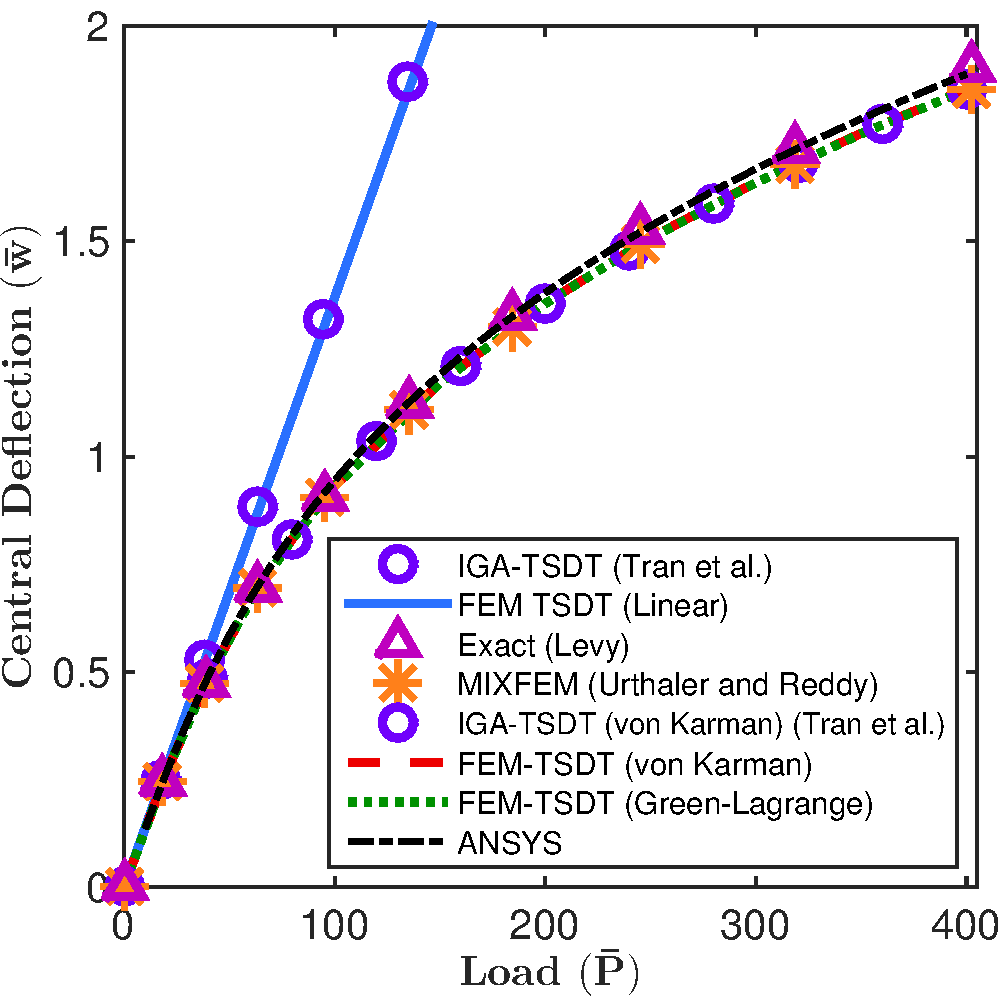
\includegraphics[scale=0.5]{Plots/Problem_NL_1}}\subfloat[\label{fig:ThinIsotropicSquarePlate_StressXX}Normalized axial stress
$\left(\bar{\sigma}_{xx}\right)$ vs load factor $\left(\bar{P}\right)$]{\centering{}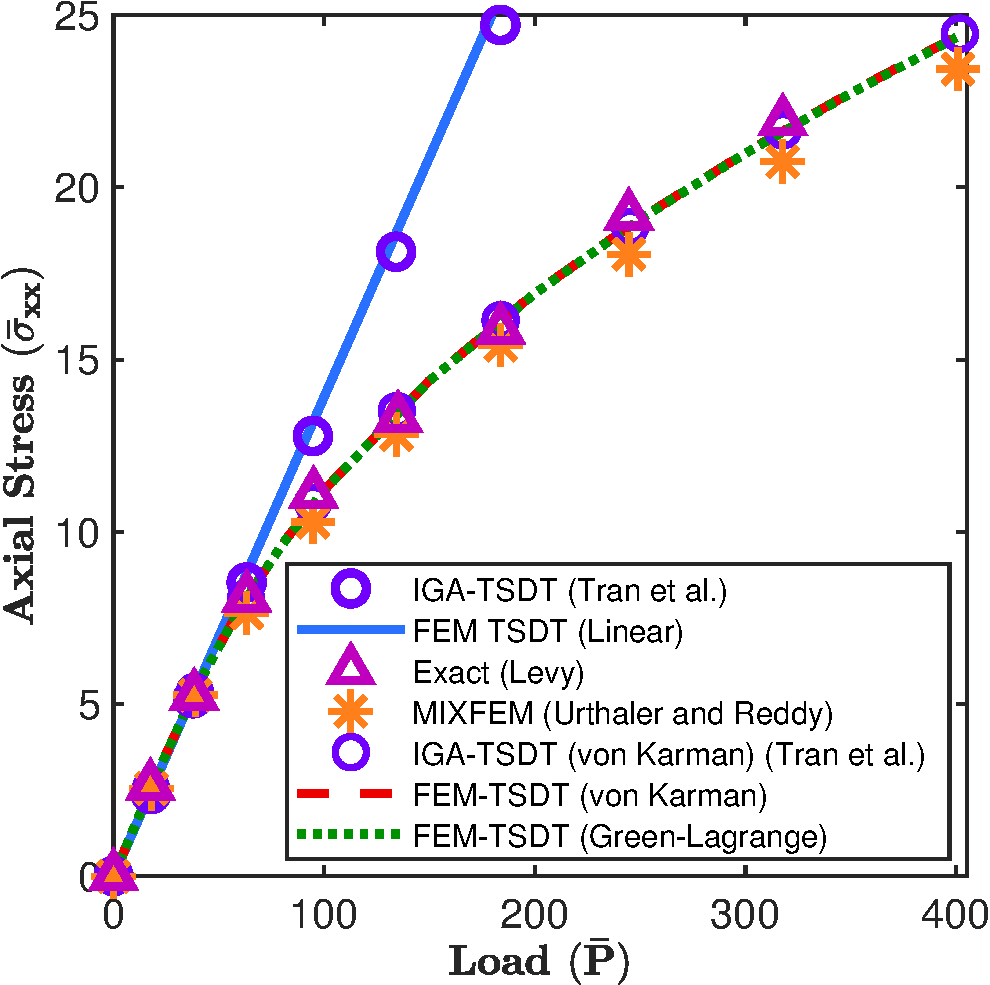
\includegraphics[scale=0.5]{Plots/Problem_NL_1_Stress_xx}}
\par\end{centering}
\caption{\label{fig:ThinIsotropicSquarePlate}Comparison of normalized central
deflection and normalized axial stress of thin isotropic clamped square
plate subjected to uniformly distributed load (UDL)}
\end{figure}
\par\end{center}

\subsubsection{Isotropic plate subjected to UDL under different type of boundary
conditions with one free edge}

Here, an isotropic square plate with in-plane dimensions, $a=b=10\,\text{in}$,
and thickness, $h=1\,\text{in}$, with material properties $E=7.8\times10^{6}\,\text{psi}$
and $\nu=0.3$ \citep{Le_Manh_2015} is considered for the nonlinear
bending analysis. The plate is subjected to uniformly distributed
load (UDL) under different set of boundary conditions. The analysis
is carried out under the consideration of von Kármán as well as Green-Lagrange
sense of strain-displacement nonlinearity, and the obtained results
are illustrated in \ref{fig:IsotropicDifferentBoundaryCondition}.
The normalized central deflections, $\bar{w}=w\left(\frac{a}{2},\frac{b}{2}\right)/h$
for $CCCC$, $SSSS2$, and $SSSS4$ boundary condition are plotted
against the load parameter, $\bar{P}=P_{0}a^{4}/Eh^{4}$ and found
to be almost same in the both nonlinear strain-displacement relations.
However, in the boundary conditions $CCFC$, $SSFS2$, $SSFS4$, a
substantial difference is observed, which in turn ascertain the utility
of Green-Lagrange strain nonlinearity in the nonlinear analysis. Also,
the central deflections obtained using Green-Lagrange nonlinearity
are found to be lower than the von Kármán results (see \ref{fig:IsotropicDifferentBoundaryCondition})
due to more terms involved in the Green-Lagrange formulation. However,
ANSYS results predict higher central deflection at large load parameter,
$\bar{P}$. The reason for this discrepancy can be attributed to the
formulation used in the ANSYS package, i.e., utilization of FSDT with
thickness stretching and other parameters along with the imposition
of boundary conditions. It is important to note that a significant
difference is observed between von Kármán and Green-Lagrange results
for $SSSS1$ and $SSFS1$ due to the contribution of normal in-plane
displacement in the nonlinear strain. This difference emphasizes the
use of Green-Lagrange strain relation for plates with one free edge.
The same emphasis is provided by the closeness of Green-Lagrange FEM
results and ANSYS results. As per authors' knowledge, this type of
novel results with their validation is not found in the literature
and can be considered benchmark results for future investigation using
Green-Lagrange nonlinearity. 
\begin{center}
\begin{figure}[H]
\begin{centering}
\subfloat[CCFC and CCCC]{\begin{centering}
\includegraphics[scale=0.5]{Plots/Problem_NL_5_0}
\par\end{centering}
}\subfloat[SSSS1 and SSFS1]{\centering{}\includegraphics[scale=0.5]{Plots/Problem_NL_5_1}}
\par\end{centering}
\centering{}\subfloat[SSSS2 and SSFS2]{\centering{}\includegraphics[scale=0.5]{Plots/Problem_NL_5_2}}\subfloat[SSSS4 and SSFS4]{\centering{}\includegraphics[scale=0.5]{Plots/Problem_NL_5_4}}\caption{\label{fig:IsotropicDifferentBoundaryCondition}Load-deflection curves
of square isotropic plate subjected to uniformly distributed load
(UDL) under different set of boundary conditions with $a/h=10$}
\end{figure}
\par\end{center}

\subsubsection{Orthotropic and four-layered square laminated plates under UDL}

Particularly, this set of problems is considered as the benchmark
problem for the validation of the laminated composite plate. In the
first part, a simply supported $\left(SSSS1\right)$ square orthotropic
plate with material properties $Material-III$ \citep{Zaghloul_1975,Tran_2015},
under uniformly distributed load (UDL), is considered. The plate dimensions
are $a=b=12\,\text{in}$ and $h=0.138\,\text{in}$. In second part,
a four-layered $\left(0^{0}/90^{0}/90^{0}/0^{0}\right)$ square laminated
plate under uniformly distributed load (UDL) with material properties
$Material-IV$ is studied with $a=b=12\,\text{in}$ and $h=0.096\,\text{in}$.
\Cref{fig:Orthotropic_0_90_90_0} reveals that the present FEM results
are found to be well-matched with IGA-TSDT results of Tran et al.
\citep{Tran_2015} which validate our formulation for the laminated
composite plate. However, in the clamped plate (in \ref{fig:Clamped_0_90_90_0}),
there is a discrepancy between experimental \citep{Zaghloul_1975}
and present FEM results. This may be attributed to inadequate clamped
boundary constraints in the experimental setup and uncertainty in
the material properties of the specimen. Moreover, the importance
of shear deformation for orthotropic material is vindicated in this
problem by the large discrepancy possessed by the finite-difference
results of CPT \citep{Zaghloul_1975}.
\begin{center}
\begin{figure}[H]
\begin{centering}
\subfloat[Simply supported orthotropic plate]{\centering{}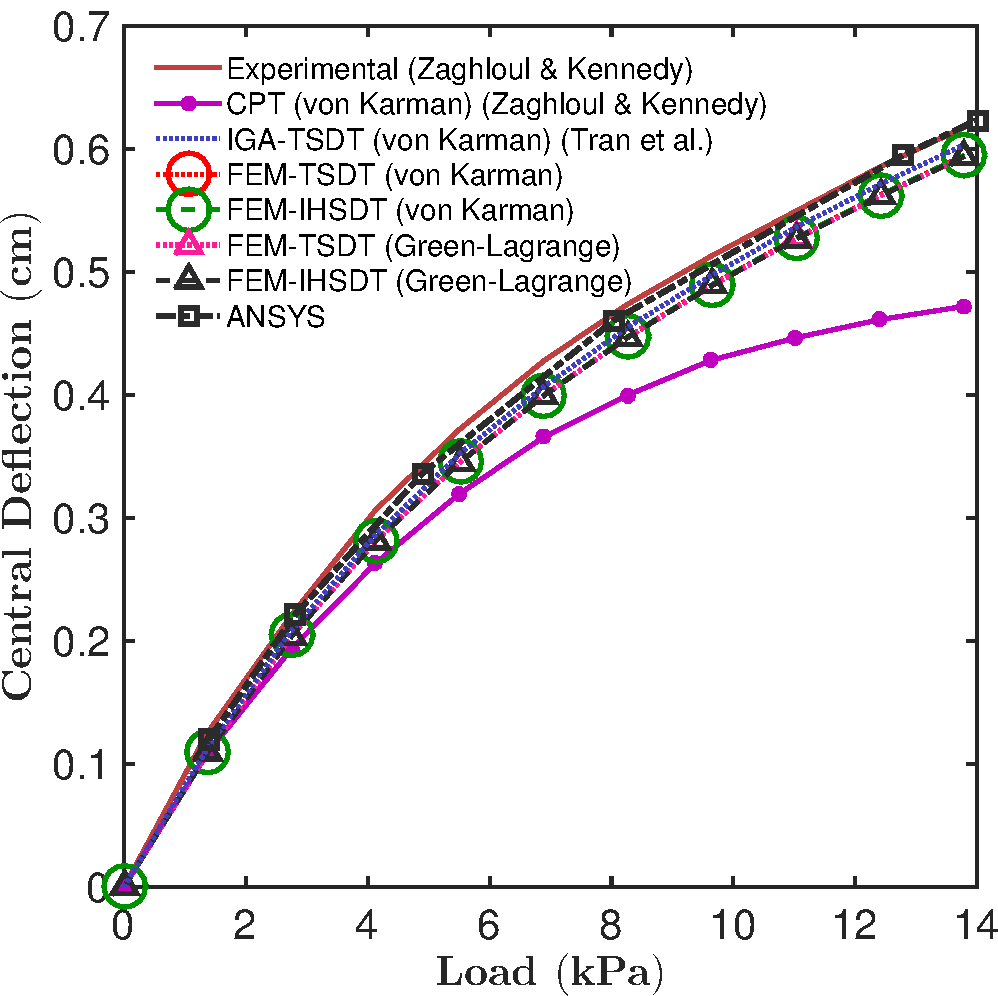
\includegraphics[scale=0.5]{Plots/Problem_NL_6_1}}\subfloat[\label{fig:Clamped_0_90_90_0}Clamped laminated plate]{\centering{}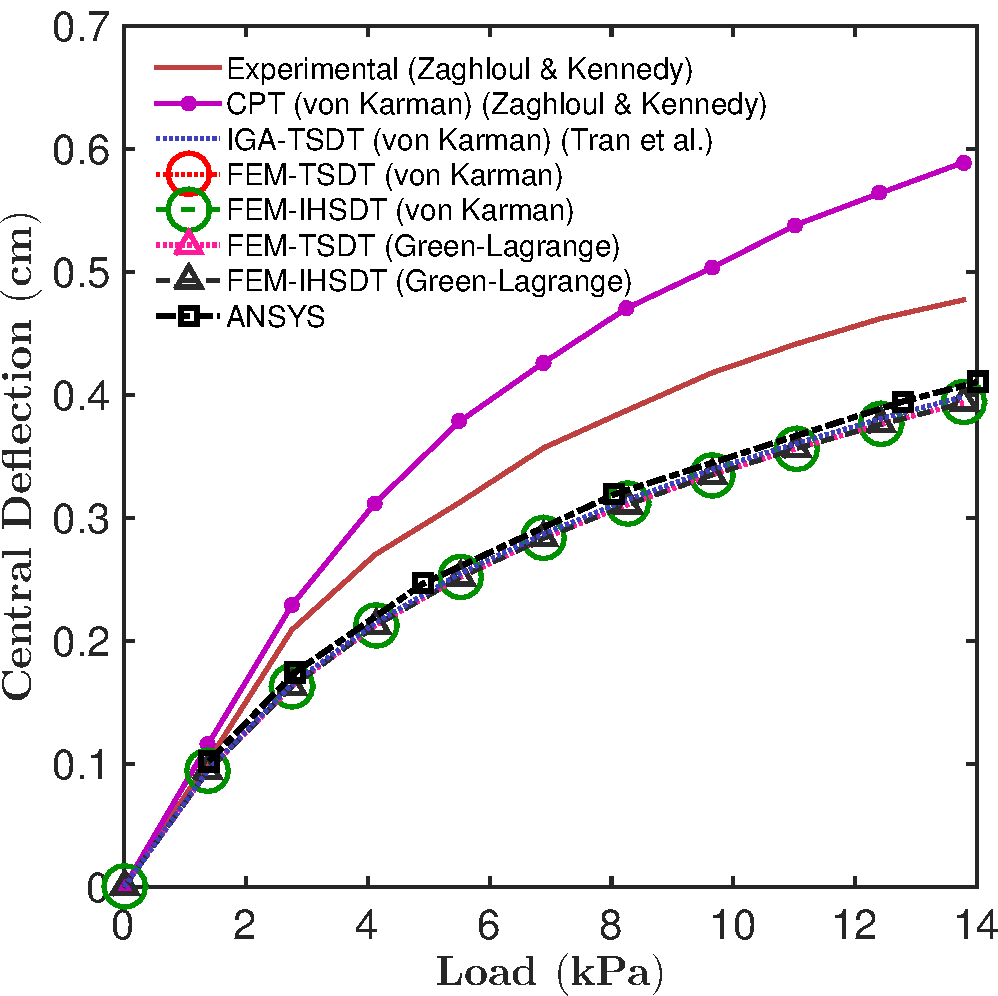
\includegraphics[scale=0.5]{Plots/Problem_NL_6_2}}
\par\end{centering}
\caption{\label{fig:Orthotropic_0_90_90_0}Load-deflection curve of (a) simply
supported square orthotropic plate (b) clamped square laminated $\left(0^{0}/90^{0}/90^{0}/0^{0}\right)$
plate under uniformly distributed load (UDL) }
\end{figure}
\par\end{center}

\subsubsection{\label{subsec:0_90_90_0}Hinged symmetric laminated plate under UDL}

In this example, a four layered $\left(0^{0}/90^{0}/90^{0}/0^{0}\right)$
square composite plate with all sides hinged $\left(SSSS3\right)$,
subjected to uniformly distributed load (UDL), is considered. Each
layer of the plate is made of $Material-I$ \citep{Le_Manh_2015}.
For comparison the normalized central deflection, $\bar{w}=w_{0}\left(\frac{a}{2},\frac{b}{2}\right)/h$
and normalized load parameter, $\bar{P}=P_{0}a^{4}/E_{2}h^{4}$ are
considered. The present FEM and ANSYS results are compared with those
available PSDT \citep{Kant_1992,Nguyen_Van_2014,Tran_2015} and NPSDT
\citep{Singh_2012} solutions and tabulated in \ref{tab:0_90_90_0_SSSS3}.\textcolor{red}{{}
}It can be observed from the \ref{tab:0_90_90_0_SSSS3} that the present
von Kármán results are matching very well with the FE solution of
Kant \citep{Kant_1992} and isogeometric results of Tran et al. \citep{Tran_2015}
for $a/h=10,\,20,\,40$. Moreover, a slightly lower deflection, around
$(1\%)$, is obtained using Green-Lagrange nonlinearity at higher
load parameter for moderately thick, $a/h=10$ plate with respect
to von Kármán results due to more nonlinear terms in the strain-displacement
relation. It is to be noted that due to the restraint of in-plane
(normal) displacements no significant difference is found between
von Kármán and Green-Lagrange results.
\begin{center}
\begin{sidewaystable}[H]
\caption{\label{tab:0_90_90_0_SSSS3}Normalized central deflection, $\bar{w}$
of simply supported $\left(SSSS3\right)$ square laminated $\left(0^{0}/90^{0}/90^{0}/0^{0}\right)$
plate subjected to uniformly distributed load (UDL)}

\centering{}\resizebox{\textwidth}{!}{%
\begin{tabular}{cccccccccccc}
\hline 
\multirow{2}{*}{$a/h$} & \multirow{2}{*}{$\bar{P}$} & $C^{0}$ HSDT$^{*}$ & MISQ20$^{*}$ & RDKQ-NL24$^{*}$ & MQRBF$^{*}$ & IGA-TSDT$^{*}$ & FEM-TSDT$^{*}$ & FEM-TSDT$^{\dagger}$ & FEM-IHSDT$^{*}$ & FEM-IHSDT$^{\dagger}$ & ANSYS\tabularnewline
 &  & \citep{Kant_1992} & \citep{Nguyen_Van_2014} & \citep{Zhang_2006} & \citep{Singh_2012} & \citep{Tran_2015} & (Present) & (Present) & (Present) & (Present) & (Present)\tabularnewline
\hline 
40 & 50 & 0.293 & 0.296 & 0.294 & 0.2654 & 0.2936 & 0.2936 & 0.2935 & 0.2940 & 0.2939 & 0.2944\tabularnewline
 & 100 & 0.464 & 0.473 & 0.467 & 0.446 & 0.4643 & 0.4643 & 0.4640 & 0.4647 & 0.4643 & 0.4649\tabularnewline
 & 150 & 0.582 & 0.592 & 0.587 & 0.616 & 0.5798 & 0.5798 & 0.5973 & 0.5801 & 0.5796 & 0.5803\tabularnewline
 & 200 & 0.664 & 0.683 & 0.679 & 0.7355 & 0.6683 & 0.6682 & 0.6675 & 0.6685 & 0.6678 & 0.6687\tabularnewline
 & 250 & 0.738 & 0.759 & 0.754 & 0.8355 & 0.7407 & 0.7408 & 0.7400 & 0.7410 & 0.7402 & 0.7414\tabularnewline
20 & 50 & 0.320 & 0.312 & 0.327 & 0.3004 & 0.3126 & 0.3126 & 0.3120 & 0.3139 & 0.3133 & 0.3149\tabularnewline
 & 100 & 0.493 & 0.487 & 0.494 & 0.5085 & 0.4807 & 0.4807 & 0.4793 & 0.4818 & 0.4804 & 0.4823\tabularnewline
 & 150 & 0.592 & 0.603 & 0.608 & 0.6591 & 0.5928 & 0.5928 & 0.5909 & 0.5937 & 0.5918 & 0.5942\tabularnewline
 & 200 & 0.680 & 0.691 & 0.695 & 0.7780 & 0.6784 & 0.6784 & 0.6760 & 0.6791 & 0.6768 & 0.6797\tabularnewline
 & 250 & 0.752 & 0.765 & 0.766 & 0.8771 & 0.7486 & 0.7486 & 0.7459 & 0.7492 & 0.7465 & 0.7500\tabularnewline
10 & 50 & 0.360 & 0.356 & 0.370 & - & 0.3609 & 0.3601 & 0.3587 & 0.3634 & 0.3613 & 0.3647\tabularnewline
 & 100 & 0.520 & 0.521 & 0.525 & - & 0.5179 & 0.5170 & 0.5141 & 0.5199 & 0.5162 & 0.5206\tabularnewline
 & 150 & 0.624 & 0.629 & 0.629 & - & 0.6213 & 0.6206 & 0.6163 & 0.6229 & 0.6181 & 0.6239\tabularnewline
 & 200 & 0.696 & 0.711 & 0.710 & - & 0.7005 & 0.6994 & 0.6947 & 0.7019 & 0.6963 & 0.7040\tabularnewline
 & 250 & 0.760 & 0.779 & 0.777 & - & 0.7659 & 0.7647 & 0.7594 & 0.7672 & 0.7608 & 0.7697\tabularnewline
\hline 
\multicolumn{11}{l}{$^{*}$present results using von Kármán nonlinearity; $^{\dagger}$present
results using Green-Lagrange nonlinearity} & \tabularnewline
\end{tabular}}
\end{sidewaystable}
\par\end{center}

\subsubsection{Simply supported symmetric cross-ply laminated plate under SSL}

The problem described in the previous \ref{subsec:0_90_90_0} is again
analyzed with simply supported boundary condition $\left(SSSS1\right)$
and sinusoidal distributed load (SSL), $P=P_{0}sin\left(\pi x/a\right)sin\left(\pi y/b\right)$,
for different span-to-thickness ratios, $a/h=4,\,10,\,20,\,100$;
and the obtained normalized central deflections, $\bar{w}=w\left(\frac{a}{2},\frac{b}{2}\right)/h$
are tabulated in \ref{tab:0_90_90_0_SSSS1}.   The results show
that a close agreement is found between IGA-TSDT solutions of Tran
et al. \citep{Tran_2015} and present FEM-TSDT solutions as both utilize
von Kármán sense of nonlinearity in their formulation. Note that,
in comparison to the hinged constraint ($SSSS3$) (shown in the previous
example), the effect of Green-Lagrange is more prominent in $SSSS1$.
The reason for this discrepancy can be attributed to the unconstrained
normal in-plane displacement in the $SSSS1$ boundary condition. It
can be observed from the \ref{tab:0_90_90_0_SSSS1} that for the plate
with $a/h=4$, the relative difference between von Kármán results
and Green-Lagrange results increases from $3\%$ to $27\%$ with increase
in load parameter, from $\bar{P}=50$ to $\bar{P}=300$. Here, the
relative difference is calculated with respect to von Kármán results.
Note that a good agreement is found between Green-Lagrange results
and ANSYS results which emphasizes the use of Green-Lagrange nonlinearity
for movable simply supported plate ($SSSS1$).
\begin{center}
\begin{table}[H]
\caption{\label{tab:0_90_90_0_SSSS1}Normalized central deflection, $\bar{w}$
of simply supported $\left(SSSS1\right)$ square laminated $\left(0^{0}/90^{0}/90^{0}/0^{0}\right)$
plate subjected to sinusoidal distributed load (SSL)}

\centering{}\resizebox{\textwidth}{!}{%
\begin{tabular}{ccccccccc}
\hline 
\multirow{2}{*}{$a/h$} & \multirow{2}{*}{$\bar{P}$} & FSDT$^{\#}$ & IGA-TSDT & FEM-TSDT$^{*}$ & FEM-TSDT$^{\dagger}$ & FEM-IHSDT$^{*}$ & FEM-IHSDT$^{\dagger}$ & ANSYS\tabularnewline
 &  & \citep{Tran_2015} & \citep{Tran_2015} & (Present) & (Present) & (Present) & (Present) & (Present)\tabularnewline
\hline 
4 & 50 & 0.6791 & 0.7198 & 0.7197 & 0.6929 & 0.7265 & 0.7015 & 0.6867\tabularnewline
 & 100 & 1.0788 & 1.1214 & 1.1217 & 1.0165 & 1.1261 & 1.0210 & 0.9522\tabularnewline
 & 200 & 1.6111 & 1.6555 & 1.6555 & 1.3216 & 1.6512 & 1.3175 & 1.1860\tabularnewline
 & 300 & 1.9877 & 2.0447 & 2.0387 & 1.4769 & 2.0283 & 1.4691 & 1.3042\tabularnewline
10 & 50 & 0.3236 & 0.3474 & 0.3474 & 0.3462 & 0.3535 & 0.3525 & 0.3624\tabularnewline
 & 100 & 0.6121 & 0.6501 & 0.6501 & 0.6433 & 0.6597 & 0.6536 & 0.6615\tabularnewline
 & 200 & 1.0667 & 1.1148 & 1.1147 & 1.0866 & 1.1264 & 1.1002 & 1.1012\tabularnewline
 & 300 & 1.4100 & 1.4612 & 1.4605 & 1.4033 & 1.4726 & 1.4176 & 1.4076\tabularnewline
20 & 50 & 0.2428 & 0.2504 & 0.2508 & 0.2507 & 0.2528 & 0.2527 & 0.2543\tabularnewline
 & 100 & 0.4734 & 0.4872 & 0.4872 & 0.4859 & 0.4907 & 0.4896 & 0.4963\tabularnewline
 & 200 & 0.8763 & 0.8960 & 0.8960 & 0.8893 & 0.9012 & 0.8951 & 0.7084\tabularnewline
 & 300 & 1.2024 & 1.2255 & 1.2250 & 1.2104 & 1.2308 & 1.2171 & 1.2232\tabularnewline
100 & 50 & 0.2150 & 0.2159 & 0.2159 & 0.2159 & 0.2160 & 0.2160 & 0.2160\tabularnewline
 & 100 & 0.4226 & 0.4243 & 0.4243 & 0.4243 & 0.4245 & 0.4244 & 0.4253\tabularnewline
 & 200 & 0.7967 & 0.7993 & 0.7987 & 0.7985 & 0.7990 & 0.7988 & 0.7986\tabularnewline
 & 300 & 1.1117 & 1.1146 & 1.1142 & 1.1137 & 1.1145 & 1.1140 & 1.1139\tabularnewline
\hline 
\multicolumn{9}{l}{$^{*}$present results using von Kármán nonlinearity; $^{\dagger}$present
results using Green-Lagrange nonlinearity}\tabularnewline
\multicolumn{9}{l}{$^{\#}$ FSDT results using MITC element \citep{Bathe_1985}}\tabularnewline
\end{tabular}}
\end{table}
\par\end{center}

\begin{center}
\par\end{center}

For span-to-thickness ratio, $a/h=10$, the through-thickness variation
of normalized stresses for same problem, under sinusoidal distributed
load (SSL), is illustrated in \ref{fig:0_90_90_0_SSL_Stresses}. As
expected, at higher load, $\bar{P}$ nonlinearity due to strain-displacement
is dominated, i.e., for the same normalized external load, lower normalized
stresses are developed. It is important to emphasize that as load
increases, asymmetry in the through-thickness distribution dominates
in the in-plane stresses, $\bar{\sigma}_{xx}$, $\bar{\sigma}_{yy}$,
and $\bar{\tau}_{xy}$, but symmetry retains in the transverse shear
stresses, $\bar{\tau}_{yz}$ and $\bar{\tau}_{xz}$ as same has been
observed by Tran et al. \citep{Tran_2015}. Further, an asymmetry
is observed in the through-thickness variation of in-plane stresses
due to Green-Lagrange nonlinearity. \textcolor{magenta}{Moreover,
the traction free boundary condition, which should be satisfied in
3D equilibrium, is satisfied only in linear and von Kármán nonlinearity
cases. The reason for this is the assumed traction free condition
initially imposed in linear strain tensor which retains in von Kármán
strain-displacement relation and constitutive approach used for obtaining
the transverse stresses. Whereas, due to the contribution of extra
terms in the nonlinear transverse strain components, this traction
free boundary condition is relaxed in the Green-Lagrange results.
Thus, the traction free boundary condition imposed during linear analysis
remains valid in von Kármán nonlinearity but not in Green-Lagrange
nonlinearity. It is to be noted that no stress recovery technique
is used in thickness direction and transverse stresses are obtained
through constitutive relation which leads to non-zero traction condition.
Hence, it is recommended that the use of constitutive relation for
transverse stresses should be limited to linear and von Kármán nonlinearity.
While, a 3D equilibrium approach \citep{Tornabene_2016,Tornabene_2017,Daniel_2020}
must be used in thickness direction while considering the Green-Lagrange
non-linearity. As per authors' knowledge, this types of observations
have not been reported in the available literature.}
\begin{center}
\begin{figure}[H]
\begin{centering}
\subfloat[$\bar{\sigma}_{xx}$]{\begin{centering}
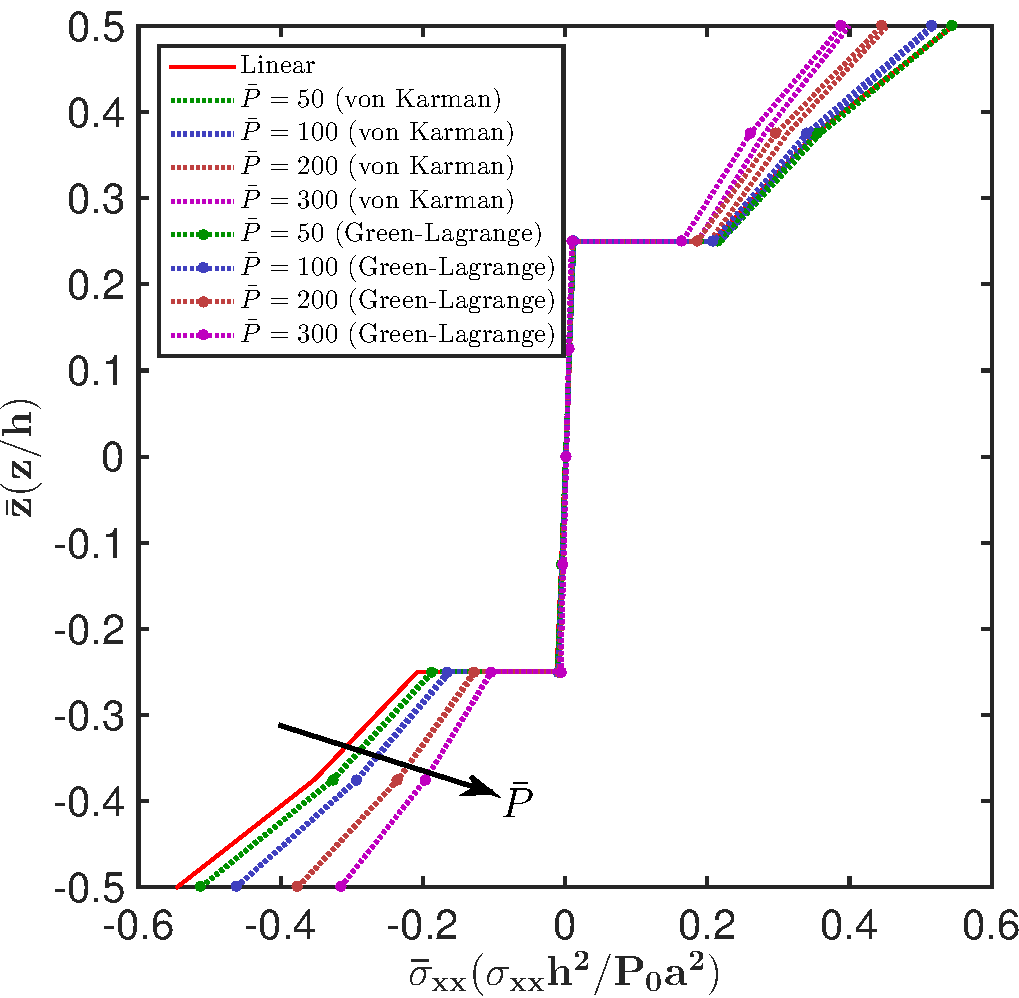
\includegraphics[scale=0.4]{Plots/Problem_NL_8_1_0_90_90_0}
\par\end{centering}
}\subfloat[$\bar{\sigma}_{yy}$]{\centering{}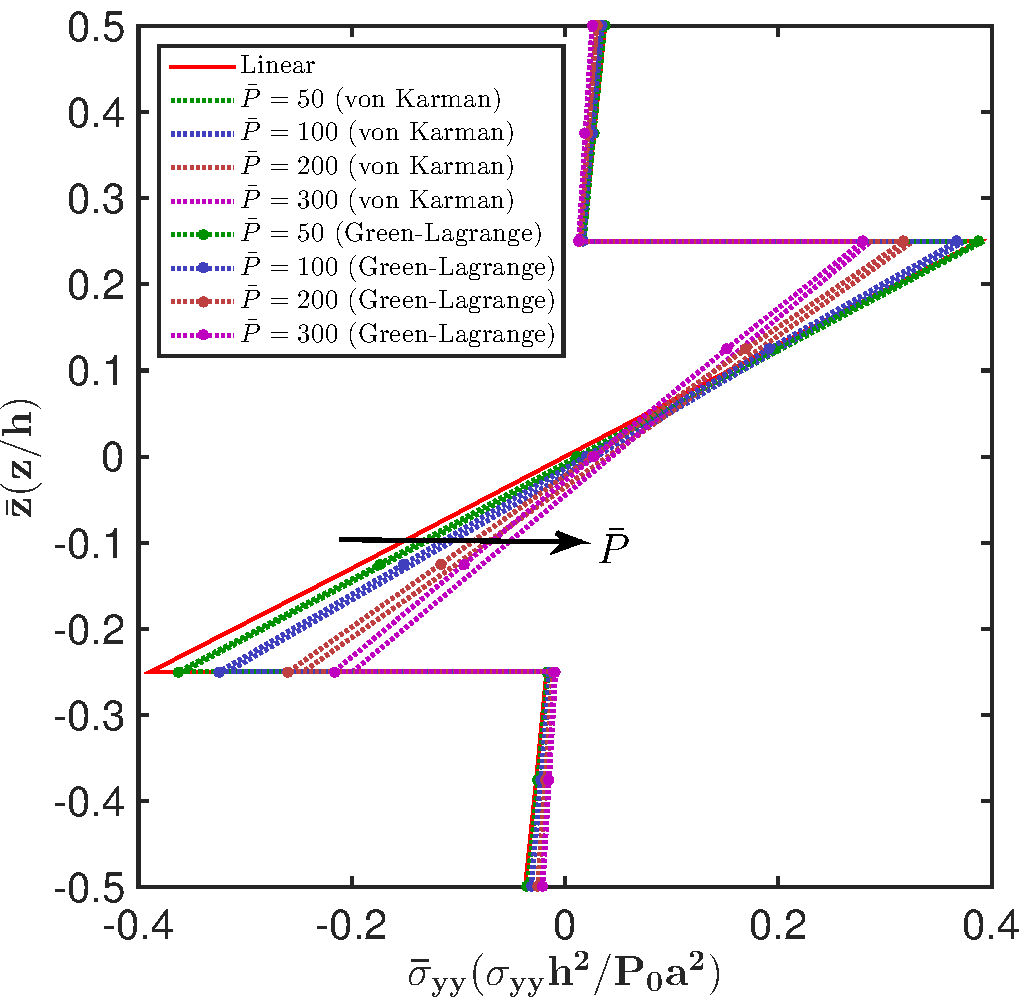
\includegraphics[scale=0.4]{Plots/Problem_NL_8_2_0_90_90_0}}
\par\end{centering}
\begin{centering}
\subfloat[$\bar{\tau}_{yz}$]{\centering{}\includegraphics[scale=0.41]{Plots/Problem_NL_8_4_0_90_90_0}}\subfloat[$\bar{\tau}_{xz}$]{\centering{}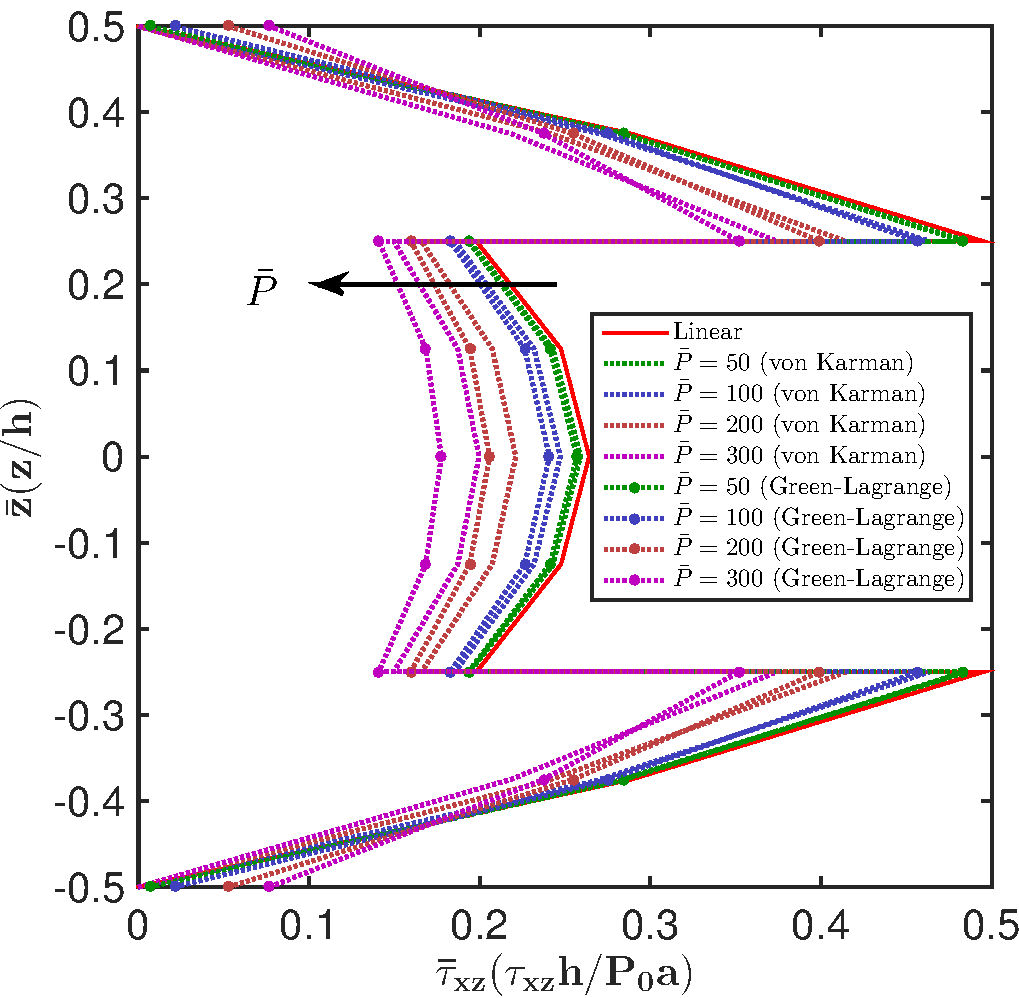
\includegraphics[scale=0.41]{Plots/Problem_NL_8_5_0_90_90_0}}
\par\end{centering}
\begin{centering}
\subfloat[$\bar{\tau}_{xy}$]{\centering{}\includegraphics[scale=0.4]{Plots/Problem_NL_8_3_0_90_90_0}}
\par\end{centering}
\caption{\label{fig:0_90_90_0_SSL_Stresses}Effect of increasing load parameter
$\bar{P}$ on through thickness distribution of stresses of simply
supported $\left(SSSS1\right)$ square laminated $\left(0^{0}/90^{0}/90^{0}/0^{0}\right)$
plate subjected to sinusoidal distributed load (SSL) with $a/h=10$:
the curves corresponding to load parameters, $\bar{P}=$ 50, 100,
200, and 300 are represented in green, blue, brown, and purple, respectively}
\end{figure}
\par\end{center}

\subsubsection{Effect of penalty parameter on nonlinear bending response of anti-symmetric
cross-ply square plate under SSL}

In this example, the effect of the penalty parameter, $\gamma$ on
the geometrically nonlinear bending analysis incorporating both von
Kármán and Green-Lagrange sense of nonlinearity is investigated. To
demonstrate this, a simply supported $\left(SSSS1\right)$ anti-symmetric
cross-ply square laminated plate subjected to sinusoidal distributed
load (SSL) is considered with each ply made of $Material-II$ \citep{Reddy_2004}.
\Cref{tab:0_90_n_Penalty} shows that as load increases the effect
of penalty become significant in thick plate, $a/h=4$, in comparison
to thin plate, $a/h=100$. For instance, the relative difference due
to the effect of penalty parameter for $\left(0^{0}/90^{0}\right)$
plate is found to be around $1.9\%$ for von Kármán TSDT, $3.8\%$
Green-Lagrange TSDT, $3.8\%$ for von Kármán IHSDT, and $4.6\%$ for
Green-Lagrange IHSDT with respect to solutions at $\gamma=10^{7}$
for $\bar{P}=300$. It is to be noticed that in this example a material
with higher orthotropic nature is considered i.e., $E_{1}/E_{2}=40$
in comparison to previous problems where $E_{1}/E_{2}=25$. Moreover,
this relative difference increases with the load parameter, $\bar{P}$.
Thus, the effect of penalty stiffness is important for those plates
which possess strong extensional-bending coupling and decreases as
the number of layers increases. Similar to the linear analysis of
anti-symmetric cross-ply, here also, the performance of TSDT is found
to be marginally better than IHSDT. Note that a good agreement is
found between Green-Lagrange results and ANSYS results. However, a
little discrepancy is found, which can be due to the formulation used
in the ANSYS package, i.e., FSDT with thickness stretching effect,
and convergence and tolerance parameter utilized in it. 
\begin{center}
\begin{table}[H]
\caption{\label{tab:0_90_n_Penalty}Effect of penalty parameter on normalized
central deflection, $\bar{w}$ of simply supported $\left(SSSS1\right)$
anti-symmetric cross-ply $\left(0^{0}/90^{0}\right)_{n}$ laminated
plate subjected to sinusoidal distributed load (SSL)}

\centering{}\resizebox{\textwidth}{!}{%
\begin{tabular}{cccccccccccc}
\hline 
\multirow{2}{*}{$n$} & \multirow{2}{*}{$a/h$} & \multirow{2}{*}{$\bar{P}$} & \multicolumn{2}{l}{FEM-TSDT$^{*}$} & \multicolumn{2}{l}{FEM-TSDT$^{\dagger}$} & \multicolumn{2}{l}{FEM-IHSDT$^{*}$} & \multicolumn{2}{l}{FEM-IHSDT$^{\dagger}$} & ANSYS\tabularnewline
\cline{4-12} \cline{5-12} \cline{6-12} \cline{7-12} \cline{8-12} \cline{9-12} \cline{10-12} \cline{11-12} \cline{12-12} 
 &  &  & $\gamma=10^{7}$ & $\gamma=0$ & $\gamma=10^{7}$ & $\gamma=0$ & $\gamma=10^{7}$ & $\gamma=0$ & $\gamma=10^{7}$ & $\gamma=0$ & (Present)\tabularnewline
\hline 
1 & 4 & 50 & 0.5808 & 0.5883 & 0.5606 & 0.5655 & 0.5594 & 0.5845 & 0.5450 & 0.5621 & 0.6231\tabularnewline
 &  & 100 & 0.9484 & 0.9582 & 0.8703 & 0.8780 & 0.9241 & 0.9542 & 0.8589 & 0.8751 & 0.8959\tabularnewline
 &  & 200 & 1.4306 & 1.4499 & 1.2242 & 1.2481 & 1.4004 & 1.4457 & 1.2157 & 1.2500 & 1.1547\tabularnewline
 &  & 300 & 1.7776 & 1.8112 & 1.4052 & 1.4585 & 1.7397 & 1.8067 & 1.3920 & 1.4564 & 1.2974\tabularnewline
 & 100 & 50 & 0.3759 & 0.3759 & 0.3759 & 0.3758 & 0.3758 & 0.3758 & 0.3758 & 0.3758 & 0.3822\tabularnewline
 &  & 100 & 0.6877 & 0.6877 & 0.6876 & 0.6876 & 0.6876 & 0.6877 & 0.6875 & 0.6875 & 0.6857\tabularnewline
 &  & 200 & 1.1382 & 1.1382 & 1.1378 & 1.1378 & 1.1381 & 1.1381 & 1.1377 & 1.1378 & 1.1355\tabularnewline
 &  & 300 & 1.4581 & 1.4581 & 1.4574 & 1.4575 & 1.4580 & 1.4581 & 1.4574 & 1.4575 & 1.4580\tabularnewline
3 & 4 & 50 & 0.4554 & 0.4555 & 0.4498 & 0.4503 & 0.4450 & 0.4521 & 0.4418 & 0.4470 & 0.4638\tabularnewline
 &  & 100 & 0.7922 & 0.7926 & 0.7627 & 0.7670 & 0.7788 & 0.7882 & 0.7571 & 0.7874 & 0.7336\tabularnewline
 &  & 200 & 1.2603 & 1.2647 & 1.1644 & 1.1660 & 1.2419 & 1.2595 & 1.1374 & 1.1654 & 1.0109\tabularnewline
 &  & 300 & 1.6038 & 1.6167 & 1.3391 & 1.3502 & 1.5786 & 1.6108 & 1.3429 & 1.3578 & 1.1546\tabularnewline
 & 100 & 50 & 0.1511 & 0.1511 & 0.1511 & 0.1511 & 0.1511 & 0.1511 & 0.1511 & 0.1511 & 0.1505\tabularnewline
 &  & 100 & 0.2999 & 0.2999 & 0.2999 & 0.2999 & 0.2999 & 0.2999 & 0.2999 & 0.2999 & 0.2989\tabularnewline
 &  & 200 & 0.5832 & 0.5832 & 0.5831 & 0.5831 & 0.5832 & 0.5832 & 0.5831 & 0.5831 & 0.5818\tabularnewline
 &  & 300 & 0.8412 & 0.8411 & 0.8409 & 0.8409 & 0.8411 & 0.8411 & 0.8409 & 0.8409 & 0.8389\tabularnewline
\hline 
\multicolumn{12}{l}{$^{*}$present results using von Kármán nonlinearity; $^{\dagger}$present
results using Green-Lagrange nonlinearity}\tabularnewline
\hline 
\end{tabular}}
\end{table}
\par\end{center}

\subsubsection{Laminated composite plate subjected to UDL under different boundary
conditions with one free edge }

In this example, a laminated composite plate with one free edge subjected
to uniformly distributed load (UDL) is considered for nonlinear analysis.
The other three edges are subjected to a different set of boundary
conditions. For this study, a square laminated plate ($a=b=10\,\text{in}$)
having material properties $Material-I$ \citep{Le_Manh_2015} with
$E_{2}=10^{6}\,\text{psi}$ is taken for parametric study. In \ref{fig:Laminated_Different_BC_a_h}
the effect of different boundary conditions $SSSS1$ and $SSFS1$
for thick, $a/h=4$ and thin, $a/h=50$ for symmetric four-layered
$\left(0^{0}/90^{0}/90^{0}/0^{0}\right)$ laminated composite plate
is illustrated. It is observed that in the case of all simply supported
($SSSS1$) edges, von Kármán and Green-Lagrange solutions agree quite
well for $a/h=50$. However, in the case of a $SSFS1$ boundary condition
distinguishable response is observed due to the significant contribution
of Green-Lagrange strain term with an increase in the value of load
parameter, $\bar{P}=P_{0}a^{4}/E_{2}h^{4}$. Moreover, the difference
increases (with respect to normalized load parameter, $\bar{P}$)
as the plate become thicker. \Cref{fig:Laminated_Different_BC_Number_Of_Layers}
emphasizes that as the number of layers increases, the discrepancy
between von Kármán and Green-Lagrange results, for $SSFS1$ boundary
condition, decreases due to the vanishing of bending-extensional coupling.
\Cref{fig:Laminated_Different_Fiber_Orientation} shows that, in
comparison with $\left(45^{0}/-45^{0}\right)_{2}$, a large discrepancy
between von Kármán and Green-Lagrange results is found with $\left(0^{0}/90^{0}\right)_{2}$
lamination.   The reason for this discrepancy can be attributed
to high magnitude of bending-extension coupling possesses by anti-symmetric
cross-ply lamination with lower bending stiffness matrix. Note that,
in all different cases, ANSYS results are also plotted, which shows
a reasonably good agreement with Green-Lagrange results and highlights
the importance of Green-Lagrange nonlinearity over von Kármán nonlinearity. 
\begin{center}
\begin{figure}[H]
\begin{centering}
\subfloat[\label{fig:Laminated_Different_BC_a_h}Effect of span-to-thickness
ratio]{\centering{}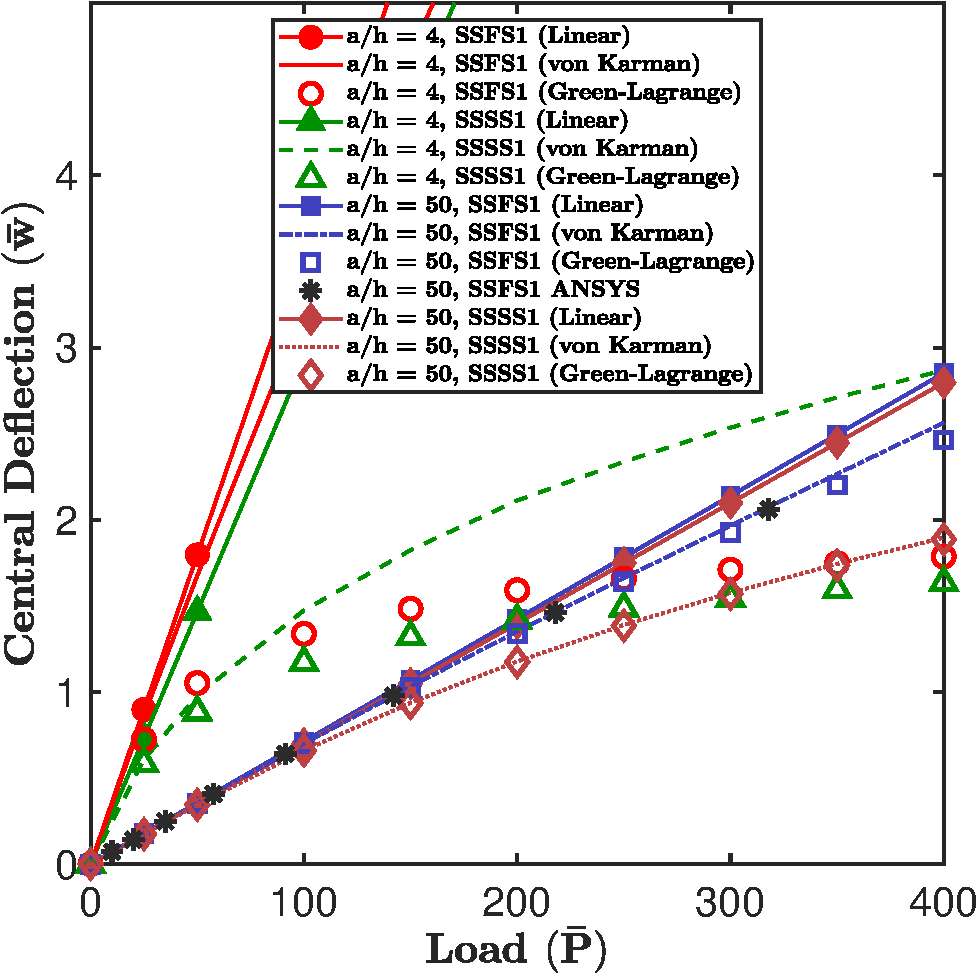
\includegraphics[scale=0.5]{Plots/Problem_NL_10_1}}\subfloat[\label{fig:Laminated_Different_BC_Number_Of_Layers}Effect of number
of layers for $a/h=20$]{\centering{}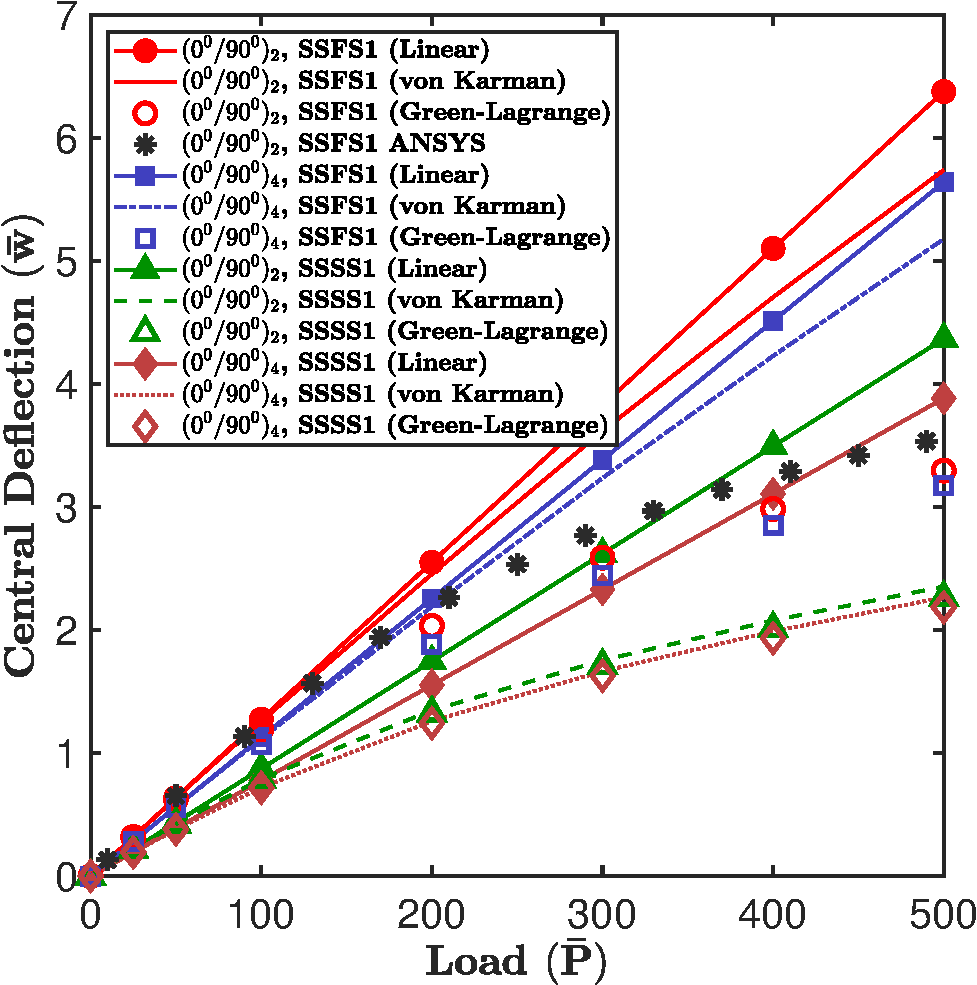
\includegraphics[scale=0.5]{Plots/Problem_NL_10_2}}
\par\end{centering}
\centering{}\subfloat[\label{fig:Laminated_Different_Fiber_Orientation}Effect of fiber
orientation for $a/h=20$]{\centering{}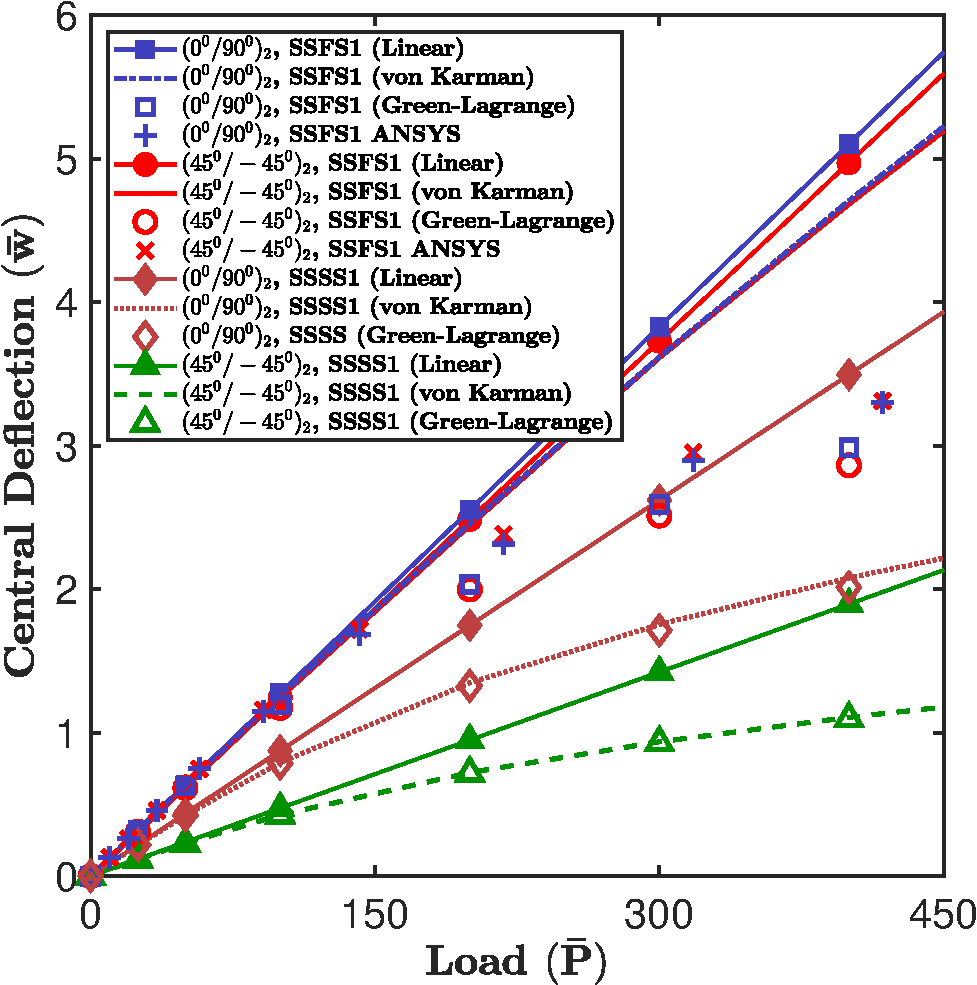
\includegraphics[scale=0.5]{Plots/Problem_NL_10_3}}\caption{\label{fig:Laminated_Different_BC}Effect of span-to-thickness ratio,
number of layers, and fiber orientation on load-deflection curve of
square laminated plate with one free edge subjected to uniformly distributed
load (UDL)}
\end{figure}
\par\end{center}

\subsubsection{Simply supported anti-symmetric cross-ply and angle-ply laminated
plates under UDL}

In this example, a simply supported $\left(SSSS1\right)$ square laminated
plate with $Material-II$ \citep{Reddy_2004}, under uniformly distributed
load (UDL), is considered for parametric study. The results are obtained
to assess the influence of the number of layers on the nonlinear bending
response of plate with $a/h=4$ and $10$, and the same is shown in
\ref{fig:NumberOfLayers_0_90_n}. It can be observed from the \ref{fig:NumberOfLayers_0_90_n}
that as the number of layers increases, the effect of nonlinearity
decreases as depicted from the difference between linear and nonlinear
results. Moreover, the effect of nonlinearity is more prominent in
a thick plate, $a/h=4$. Furthermore, a small difference is observed
between von Kármán and Green-Lagrange nonlinearity for the moderately
thick plate, $a/h=10$. 
\begin{center}
\begin{figure}[H]
\centering{}\subfloat[$a/h=10$]{\centering{}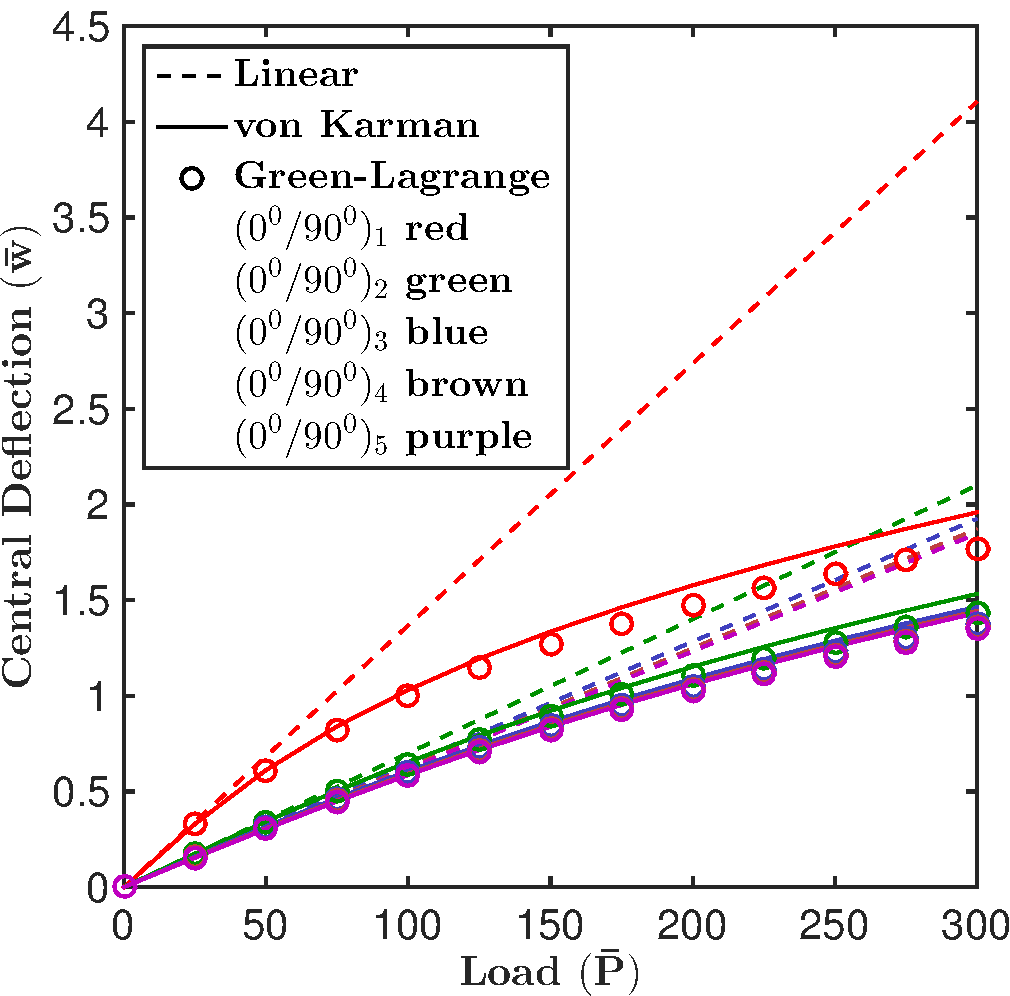
\includegraphics[scale=0.5]{Plots/Problem_NL_9_1_1}}\subfloat[$a/h=4$]{\centering{}\includegraphics[scale=0.5]{Plots/Problem_NL_9_1_2}}\caption{\label{fig:NumberOfLayers_0_90_n}Effect of number of layers on load-deflection
curve of simply supported $\left(SSSS1\right)$ cross-ply $\left(0^{0}/90^{0}\right)_{n}$
laminatedplate subjected to uniformly distributed load (UDL) with
$a/h=10$ and $a/h=4$}
\end{figure}
\par\end{center}

In \ref{fig:Effect_of_fiber_Orientation}, the effect of the fiber
orientation on the bending response of anti-symmetric angle-ply $\left(-\theta/\theta/-\theta/\theta\right)$
plate is shown. Here, it can be observed that the difference between
linear and nonlinear is constant for various anti-symmetric angle-ply
plates for $a/h=10$. This difference implies that as the fiber angle
increases, only bending characteristic increases, leading to lower
the central deflection. Moreover, the effect of nonlinearity is prominent
in thick plates, $a/h=4$, i.e., a significant difference is observed
between linear and nonlinear characteristics of plate with $a/h=10$. 
\begin{center}
\begin{figure}[H]
\centering{}\subfloat[$a/h=10$]{\centering{}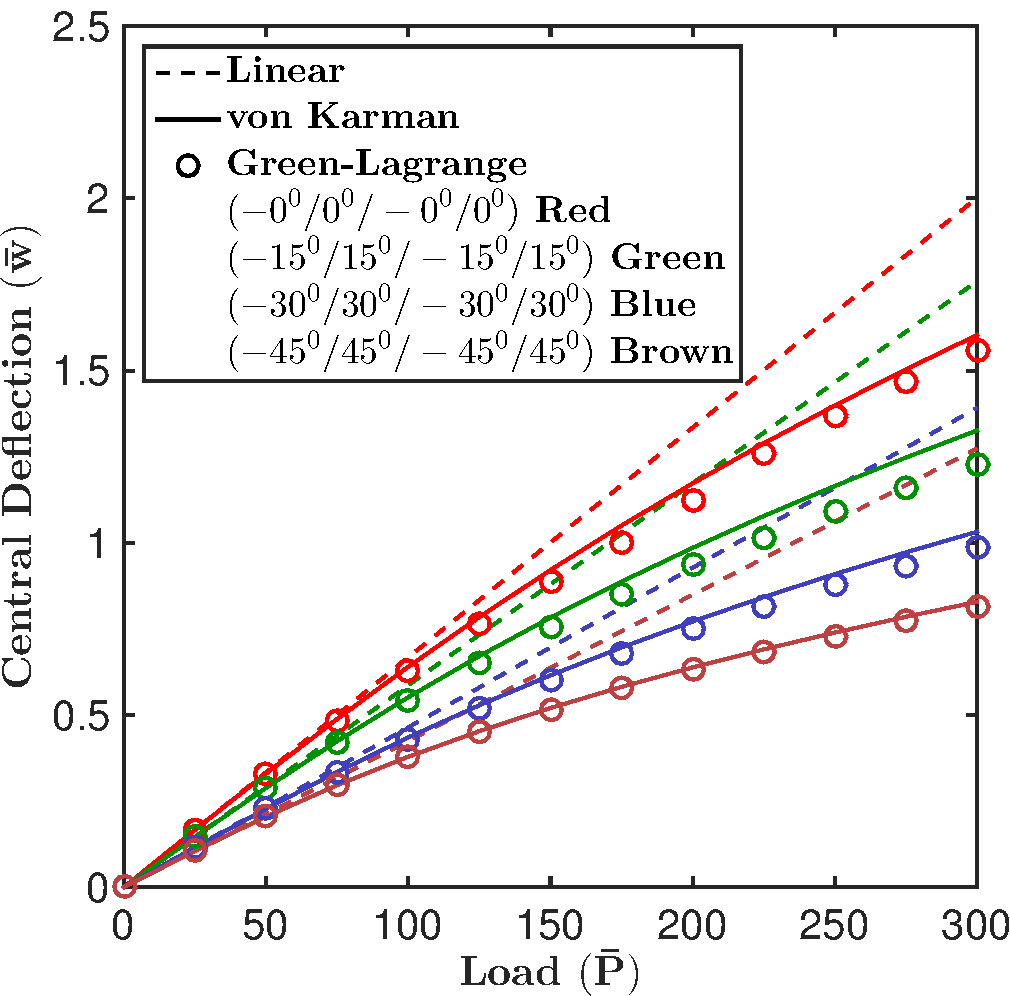
\includegraphics[scale=0.5]{Plots/Problem_NL_9_2_1}}\subfloat[$a/h=4$]{\centering{}\includegraphics[scale=0.5]{Plots/Problem_NL_9_2_2}}\caption{\label{fig:Effect_of_fiber_Orientation}Effect of fiber orientation
on load-deflection curves of simply supported $\left(SSSS1\right)$
anti-symmetric angle-ply $\left(-\theta/\theta/-\theta/\theta\right)$
laminated plate subjected to uniformly distributed load (UDL) with
$a/h=10$ and $a/h=4$}
\end{figure}
\par\end{center}

In \ref{fig:Symmetric_antisymmetric_AnglePly}, the variation of normalized
central deflection with fiber orientation of symmetric and anti-symmetric
angle-ply composite plate is illustrated. It is found that fiber with
$45^{0}$ orientation is optimal for design, and anti-symmetric angle-ply
possesses marginally more bending stiffness than the symmetric angle-ply
plate. It is to be noted that here in this set of examples, the $SSSS1$
boundary condition is considered.
\begin{center}
\begin{figure}[H]
\centering{}\subfloat[$a/h=10$]{\begin{centering}
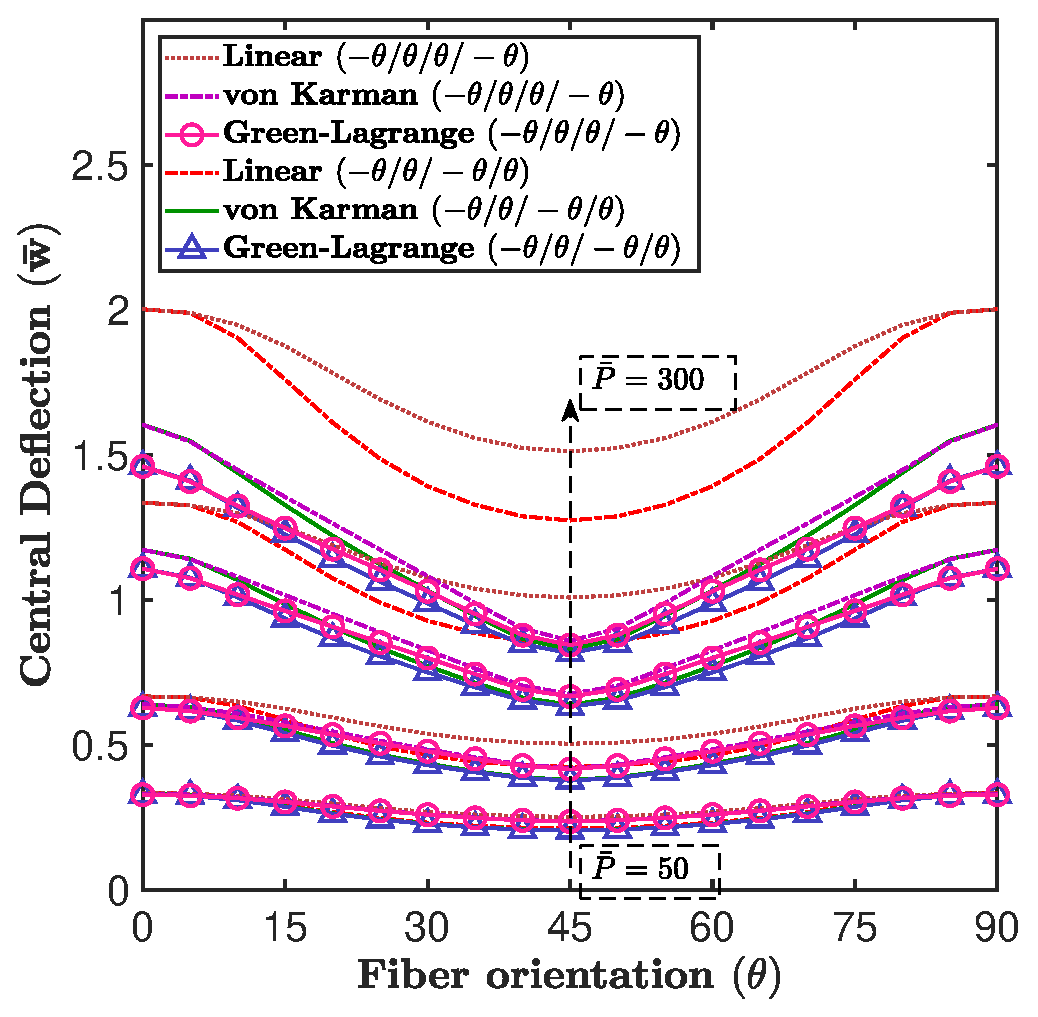
\includegraphics[scale=0.5]{Plots/Problem_NL_9_3_1}
\par\end{centering}
}\subfloat[$a/h=4$]{\begin{centering}
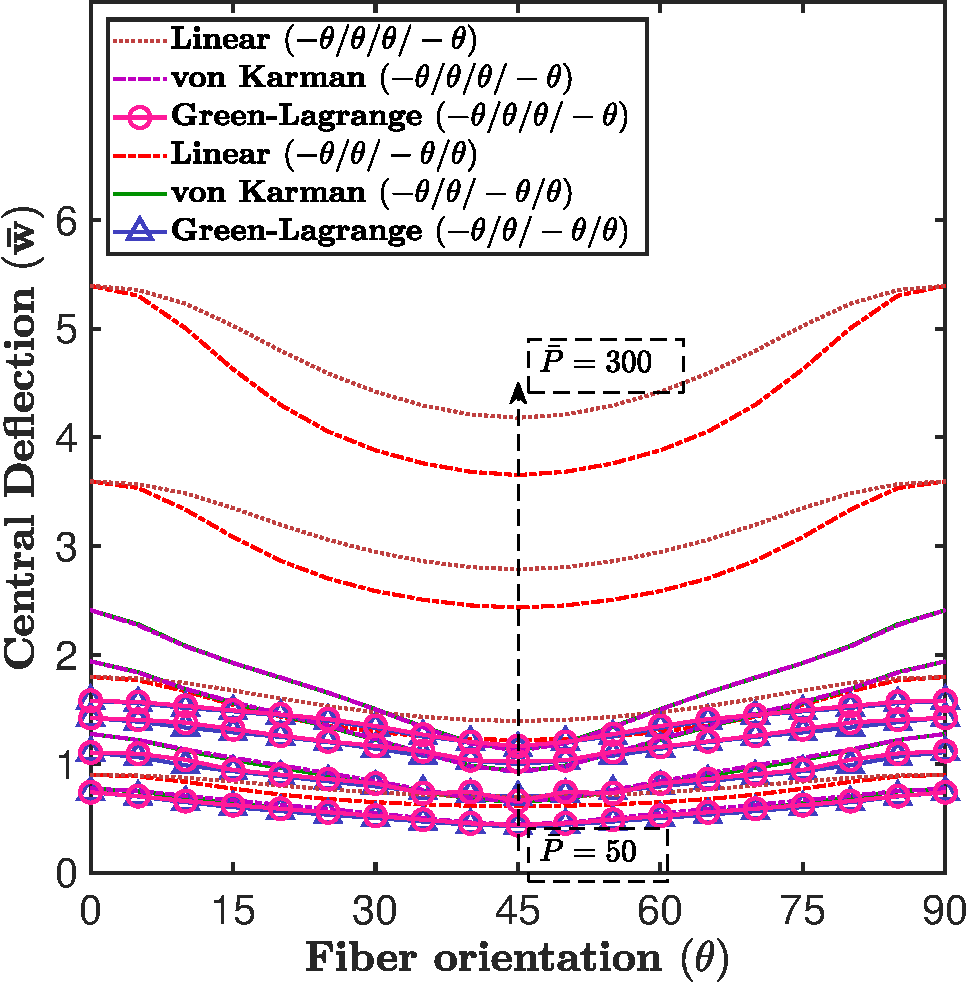
\includegraphics[scale=0.5]{Plots/Problem_NL_9_3_2}
\par\end{centering}
}\caption{\label{fig:Symmetric_antisymmetric_AnglePly}Effect of fiber orientation
on nonlinear bending response of symmetric and anti-symmetric angle-ply
laminated plates subjected to uniformly distributed load (UDL) with
$a/h=10$ and $a/h=4$}
\end{figure}
\par\end{center}

\subsubsection{Five-layered simply supported square sandwich plate under UDL}

To demonstrate the applicability of the present $C^{0}$ finite element
model for sandwich plates, a five-layered square sandwich plate is
considered in this example for nonlinear bending analysis. The plate
is composed of five layers of $Material-V$ \citep{Ganapathi_2004,Madhukar_2013},
where the top and the bottom two layers are of equal thickness. The
top/bottom two layers form the face-sheet with thickness, $h_{f}$,
and the middle layer with thickness, $h_{c}$ forms the core of the
sandwich. The geometrically nonlinear bending behavior of the simply
supported $(SSSS4)$ five-layered $\left(0^{0}/90^{0}/C/90^{0}/0^{0}\right)$
square sandwich plate is analyzed using the IHSDT model, and the same
is compared with FEM solution of normal deformation theory by Madhukar
and Singha \citep{Madhukar_2013}. The equilibrium path of normalized
central deflection, $\bar{w}=w\left(\frac{a}{2},\frac{b}{2}\right)/h$
and normalized load parameter, $\bar{P}=P_{0}a^{4}/E_{2}h^{4}$ is
obtained for different $a/h$ ratios and $h_{c}/h_{f}$ ratios, and
the same is shown in \cref{fig:Sandwich_a_h,fig:Sandwich_hC_hF},
respectively; where $E_{2}$ is the material constant of face-sheet.
The \Cref{fig:Sandwich_a_h,fig:Sandwich_hC_hF} show that a close
agreement is found between present FEM-IHSDT solution and Madhukar
and Singha solution \citep{Madhukar_2013}, which validates the applicability
of the present finite element model for sandwich plates.
\begin{center}
\begin{figure}[H]
\begin{centering}
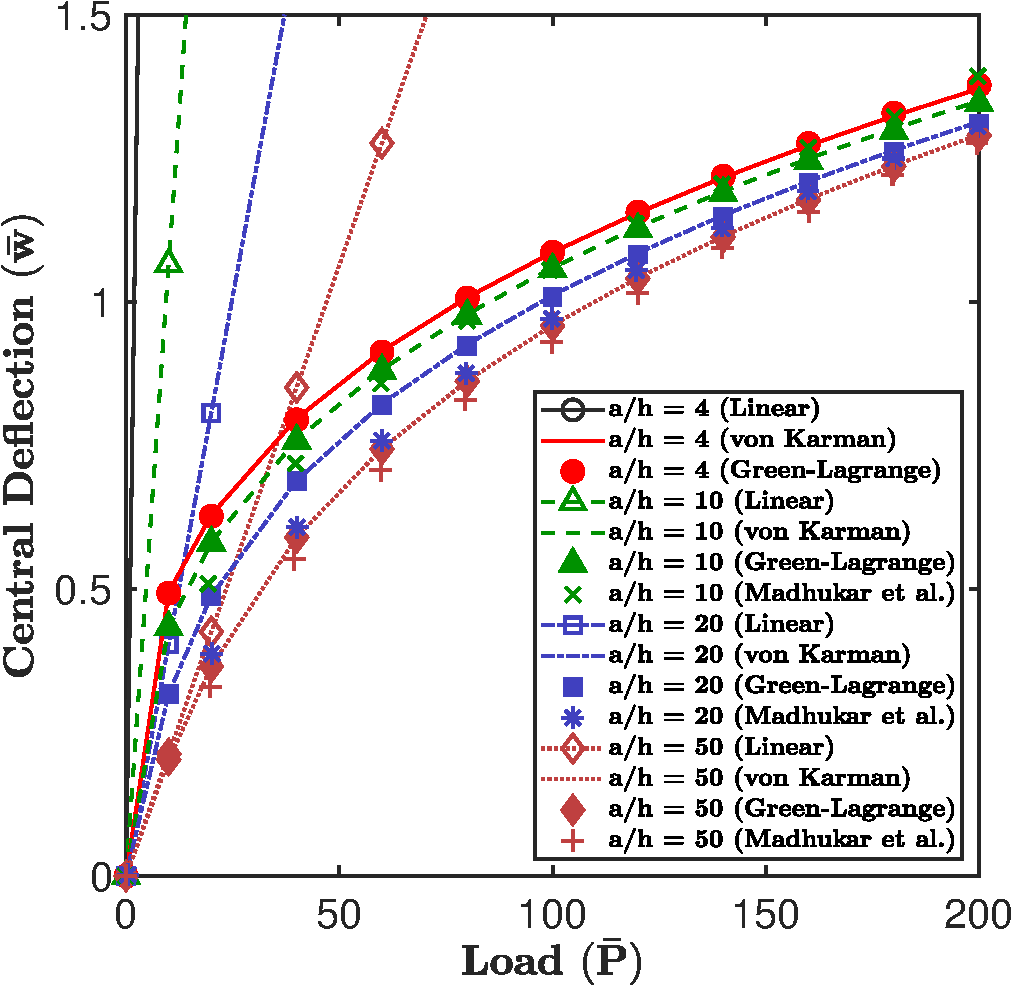
\includegraphics[scale=0.5]{Plots/Problem_NL_11_1}\caption{\label{fig:Sandwich_a_h}Effect of span-to-thickness ratio, $a/h$
on nonlinear bending response of simply supported $\left(SSSS4\right)$
square sandwich $\left(0^{0}/90^{0}/C/90^{0}/0^{0}\right)$ plate
under uniformly distributed load (UDL) with $h_{c}/h_{f}=5$}
\par\end{centering}
\end{figure}
\par\end{center}

\begin{center}
\begin{figure}[H]
\centering{}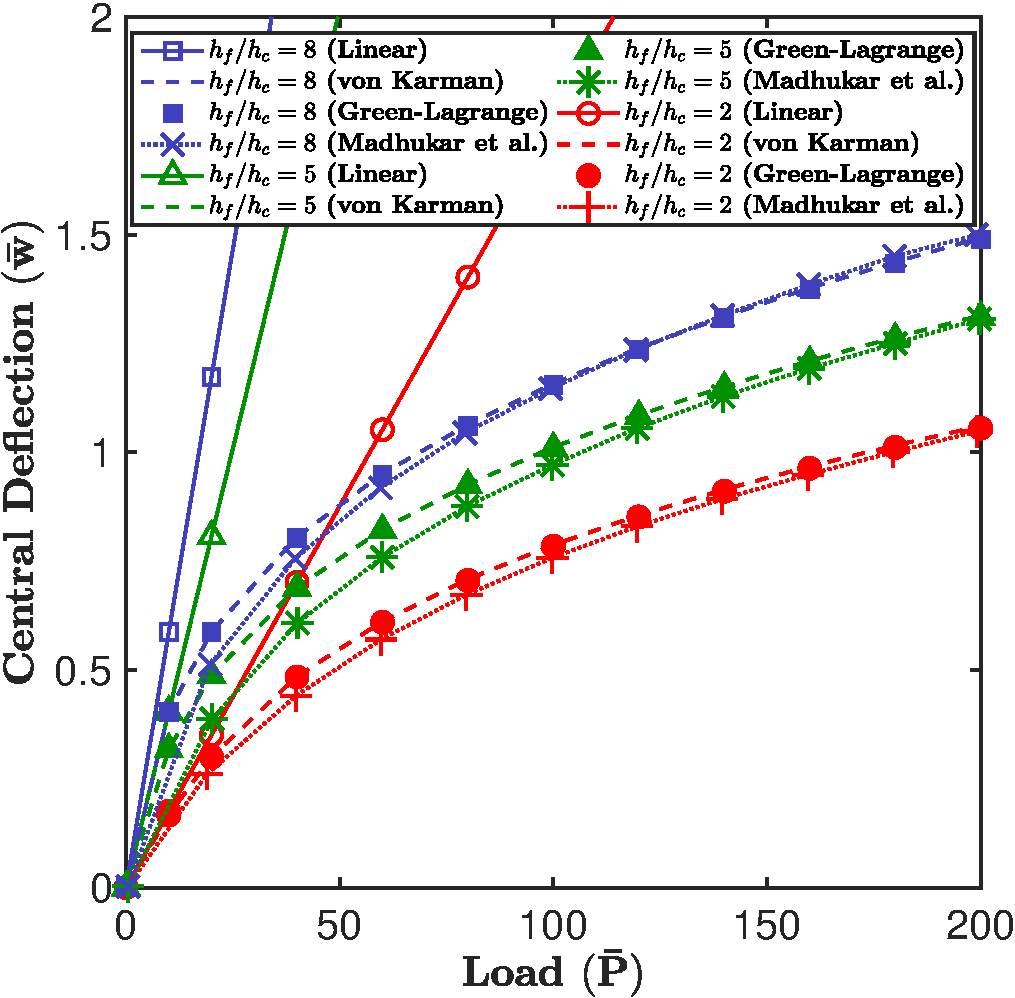
\includegraphics[scale=0.5]{Plots/Problem_NL_11_2}\caption{\label{fig:Sandwich_hC_hF}Effect of core-to-facesheet thickness ratio,
$h_{c}/h_{f}$ on nonlinear bending response of simply supported $\left(SSSS4\right)$
square sandwich $\left(0^{0}/90^{0}/C/90^{0}/0^{0}\right)$ plate
under uniformly distributed load (UDL) with $a/h=20$}
\end{figure}
\par\end{center}

\section{Conclusion\label{sec:Concluding-remarks}}

In this paper, the importance of Green-Lagrange nonlinearity over
von Kármán nonlinearity is highlighted via means of employing a $C^{0}$
finite element plate model for linear and nonlinear bending analysis
using higher-order shear deformation theories (HSDTs). The importance
of penalty consideration is also emphasized as it is revealed that
this plays a crucial role in securing a more accurate solution in
some cases.

A nine-noded $C^{0}$ finite element model with the consideration
of penalty constraints is formulated for the bending analysis of isotropic,
laminated, and sandwich plates. The study emphatically reveals several
facts and insights regarding the need for full geometric nonlinearity,
usage of the penalty parameter, and the superiority of deformation
theories. It is found that the neglect of the penalty parameter in
the formulation leads to substantial error in both linear and nonlinear
analysis, and to get the accurate response, the value of the penalty
parameter should be of the order of material constants. Further, the
importance of Green-Lagrange strain relation in the formulation is
highlighted through various examples, and it is observed that the
consideration of full geometric nonlinearity becomes essential for
the boundary conditions with a free edge or with movable simply supported
boundary condition ($SSSS1$). Besides, the effect of full geometric
nonlinearity and the effect of the penalty parameter are found to
be prominent in thick plates with $a/h\leq10$. \textcolor{magenta}{Further,
it was found that the traction free boundary conditions on the top
and bottom surfaces of the plate is only satisfied in linear and von
Kármán nonlinear analysis, but not in the Green-Lagrange nonlinear
analysis when obtained from constitutive approach.} Moreover, for
the moderately thick plate, $a/h=10$, the through-thickness variation
of in-plane stresses are found to be unsymmetrical. \textcolor{magenta}{Thus,
to accurately calculate the transverse stresses for the Green-Lagrange
nonlinearity, a stress recovery technique employing the equilibrium
approach must be considered for traction free boundary conditions. }

In addition, the performance of polynomial and nonpolynomial shear
deformation theories (PSDT $\&$ NPSDT) is holistically studied for
various structural parameters under the consideration of full geometric
nonlinearity. Moreover, a comparative study is carried out for various
parameters such as lamination schemes, side-to-thickness ratios, and
others. In case of bending analysis, the IHSDT is found to be performing
better for the symmetric cross-ply, whereas the TSDT is found to be
performing better for the anti-symmetric cross-ply multilayered composite
plates. The work presented in this paper provides a strong background
to delve into the wide scope of the NPSDT for the further study of
structural analysis. 

\appendix

\section{\label{sec:The-expression-of-Nb-and-Ns}The expression of $\mathbb{N}_{b}$
and $\mathbb{N}_{s}$}

\[
\mathbb{N}_{b}=\left[\begin{array}{cccccccccccccc}
N_{xx} & N_{xy} & 0 & 0 & 0 & 0 & M_{xx} & M_{xy} & 0 & 0 & P_{xx} & P_{xy} & 0 & 0\\
N_{xy} & N_{yy} & 0 & 0 & 0 & 0 & M_{xy} & M_{yy} & 0 & 0 & P_{xy} & P_{yy} & 0 & 0\\
0 & 0 & N_{xx} & N_{xy} & 0 & 0 & 0 & 0 & M_{xx} & M_{xy} & 0 & 0 & P_{xx} & P_{xy}\\
0 & 0 & N_{xy} & N_{yy} & 0 & 0 & 0 & 0 & M_{xy} & M_{yy} & 0 & 0 & P_{xy} & P_{yy}\\
0 & 0 & 0 & 0 & N_{xx} & N_{xy} & 0 & 0 & 0 & 0 & 0 & 0 & 0 & 0\\
0 & 0 & 0 & 0 & N_{xy} & N_{yy} & 0 & 0 & 0 & 0 & 0 & 0 & 0 & 0\\
M_{xx} & M_{xy} & 0 & 0 & 0 & 0 & Q_{xx} & Q_{xy} & 0 & 0 & R_{xx} & R_{xy} & 0 & 0\\
M_{xy} & M_{yy} & 0 & 0 & 0 & 0 & Q_{xy} & Q_{yy} & 0 & 0 & R_{xy} & R_{yy} & 0 & 0\\
0 & 0 & M_{xx} & M_{xy} & 0 & 0 & 0 & 0 & Q_{xx} & Q_{xy} & 0 & 0 & R_{xx} & R_{xy}\\
0 & 0 & M_{xy} & M_{yy} & 0 & 0 & 0 & 0 & Q_{xy} & Q_{yy} & 0 & 0 & R_{xy} & R_{yy}\\
P_{xx} & P_{xy} & 0 & 0 & 0 & 0 & R_{xx} & R_{xy} & 0 & 0 & S_{xx} & S_{xy} & 0 & 0\\
P_{xy} & P_{yy} & 0 & 0 & 0 & 0 & R_{xy} & R_{yy} & 0 & 0 & S_{xy} & S_{yy} & 0 & 0\\
0 & 0 & 0 & 0 & 0 & 0 & 0 & 0 & R_{xx} & R_{xy} & 0 & 0 & S_{xx} & S_{xy}\\
0 & 0 & 0 & 0 & 0 & 0 & 0 & 0 & R_{xy} & R_{yy} & 0 & 0 & S_{xy} & S_{yy}
\end{array}\right]
\]

\[
\mathbb{N}_{s}=\left[\begin{array}{cccccccccccccccc}
0 & 0 & 0 & 0 & N_{xz} & N_{yz} & 0 & 0 & M_{xz} & M_{yz} & 0 & 0 & P_{xz} & P_{yz} & 0 & 0\\
0 & 0 & 0 & 0 & 0 & 0 & N_{xz} & N_{yz} & 0 & 0 & M_{xz} & M_{yz} & 0 & 0 & P_{xz} & P_{yz}\\
0 & 0 & 0 & 0 & Q_{xz} & Q_{yz} & 0 & 0 & R_{xz} & R_{yz} & 0 & 0 & S_{xz} & S_{yz} & 0 & 0\\
0 & 0 & 0 & 0 & 0 & 0 & Q_{xz} & Q_{yz} & 0 & 0 & R_{xz} & R_{yz} & 0 & 0 & S_{xz} & S_{yz}\\
N_{xz} & 0 & Q_{xz} & 0 & 0 & 0 & 0 & 0 & 0 & 0 & 0 & 0 & 0 & 0 & 0 & 0\\
N_{yz} & 0 & Q_{yz} & 0 & 0 & 0 & 0 & 0 & 0 & 0 & 0 & 0 & 0 & 0 & 0 & 0\\
0 & N_{xz} & 0 & Q_{xz} & 0 & 0 & 0 & 0 & 0 & 0 & 0 & 0 & 0 & 0 & 0 & 0\\
0 & N_{yz} & 0 & Q_{yz} & 0 & 0 & 0 & 0 & 0 & 0 & 0 & 0 & 0 & 0 & 0 & 0\\
M_{xz} & 0 & R_{xz} & 0 & 0 & 0 & 0 & 0 & 0 & 0 & 0 & 0 & 0 & 0 & 0 & 0\\
M_{yz} & 0 & R_{yz} & 0 & 0 & 0 & 0 & 0 & 0 & 0 & 0 & 0 & 0 & 0 & 0 & 0\\
0 & M_{xz} & 0 & R_{xz} & 0 & 0 & 0 & 0 & 0 & 0 & 0 & 0 & 0 & 0 & 0 & 0\\
0 & M_{yz} & 0 & R_{yz} & 0 & 0 & 0 & 0 & 0 & 0 & 0 & 0 & 0 & 0 & 0 & 0\\
P_{xz} & 0 & S_{xz} & 0 & 0 & 0 & 0 & 0 & 0 & 0 & 0 & 0 & 0 & 0 & 0 & 0\\
P_{yz} & 0 & S_{yz} & 0 & 0 & 0 & 0 & 0 & 0 & 0 & 0 & 0 & 0 & 0 & 0 & 0\\
0 & P_{xz} & 0 & S_{xz} & 0 & 0 & 0 & 0 & 0 & 0 & 0 & 0 & 0 & 0 & 0 & 0\\
0 & P_{yz} & 0 & S_{yz} & 0 & 0 & 0 & 0 & 0 & 0 & 0 & 0 & 0 & 0 & 0 & 0
\end{array}\right]
\]


\section{\label{sec:Navier-solution}Navier solution for simply supported
$\left(SSSS1\right)$ anti-symmetric cross-ply composite plate}

\[
\begin{aligned}u_{0}= & \sum_{m=1}^{\infty}\sum_{n=1}^{\infty}U_{mn}cos\left(\alpha x\right)sin\left(\beta y\right) & v_{0}= & \sum_{m=1}^{\infty}\sum_{n=1}^{\infty}V_{mn}sin\left(\alpha x\right)cos\left(\beta y\right)\\
w_{0}= & \sum_{m=1}^{\infty}\sum_{n=1}^{\infty}W_{mn}sin\left(\alpha x\right)sin\left(\beta y\right) & \theta_{x}= & \sum_{m=1}^{\infty}\sum_{n=1}^{\infty}X_{mn}cos\left(\alpha x\right)sin\left(\beta y\right)\\
\theta_{y}= & \sum_{m=1}^{\infty}\sum_{n=1}^{\infty}Y_{mn}sin\left(\alpha x\right)cos\left(\beta y\right)
\end{aligned}
\]

\[
\left[\begin{array}{ccccc}
K_{11} & K_{12} & K_{13} & K_{14} & K_{15}\\
 & K_{22} & K_{23} & K_{24} & K_{25}\\
 &  & K_{33} & K_{34} & K_{35}\\
 & \text{sym} &  & K_{44} & K_{45}\\
 &  &  &  & K_{55}
\end{array}\right]\left\{ \begin{array}{c}
U_{mn}\\
V_{mn}\\
W_{mn}\\
X_{mn}\\
Y_{mn}
\end{array}\right\} =\left\{ \begin{array}{c}
0\\
0\\
F_{mn}\\
0\\
0
\end{array}\right\} 
\]

\begin{center}
$\begin{aligned}K_{11}= & \alpha^{2}A_{11}+\beta^{2}A_{66}\\
K_{12}= & \alpha\beta A_{12}+\alpha\beta A_{66}\\
K_{13}= & -\alpha\left(\alpha^{2}B_{11}+\beta^{2}B_{12}+2\beta^{2}B_{66}\right)\\
K_{14}= & \alpha^{2}C_{11}+\beta^{2}C_{66}\\
K_{15}= & \alpha\beta C_{12}+\alpha\beta C_{66}\\
K_{22}= & \alpha^{2}A_{66}+\beta^{2}A_{22}\\
K_{23}= & -\beta\left(\alpha^{2}B_{12}+\beta^{2}B_{22}+2\alpha^{2}B_{66}\right)\\
K_{24}= & \alpha\beta C_{12}+\alpha\beta C_{66}\\
K_{25}= & \alpha^{2}C_{66}+\beta^{2}C_{22}\\
K_{33}= & \alpha^{4}D_{11}+2\alpha^{2}\beta^{2}D_{12}+\beta^{4}D_{22}+4\alpha^{2}\beta^{2}D_{66}\\
K_{34}= & -\alpha\left(\alpha^{2}E_{11}+\beta^{2}E_{12}+2\beta^{2}E_{66}\right)\\
K_{35}= & -\beta\left(\alpha^{2}E_{12}+\beta^{2}E_{22}+2\alpha^{2}E_{66}\right)\\
K_{44}= & A_{55}+\alpha^{2}F_{11}+\beta^{2}F_{66}\\
K_{45}= & \alpha\beta F_{12}+\alpha\beta F_{66}\\
K_{55}= & A_{44}+\alpha^{2}F_{66}+\beta^{2}F_{22}
\end{aligned}
;$ $\begin{aligned}\left[A_{ij}\right]= & \int_{-h/2}^{h/2}\bar{Q}_{ij}dz\\
\left[B_{ij}\right]= & \int_{-h/2}^{h/2}z\bar{Q}_{ij}dz\\
\left[C_{ij}\right]= & \int_{-h/2}^{h/2}f\left(z\right)\bar{Q}_{ij}dz\\
\left[D_{ij}\right]= & \int_{-h/2}^{h/2}G\left(z\right)\bar{Q}_{ij}dz\\
\left[E_{ij}\right]= & \int_{-h/2}^{h/2}z^{2}\bar{Q}_{ij}dz\\
\left[F_{ij}\right]= & \int_{-h/2}^{h/2}zf\left(z\right)\bar{Q}_{ij}dz\\
i,j= & 1,2,6\\
\\
\left[A_{ij}\right]= & \int_{-h/2}^{h/2}f'\left(z\right)\bar{Q}_{ij}dz\\
i,j= & 4,5
\end{aligned}
$;
\par\end{center}

\begin{center}
$F_{mn}=\begin{cases}
P_{0} & \text{Sinusoidal distrbuted load (SSL)}\\
16P_{0}/\pi^{2}mn & \text{Uniformly distrbuted load (UDL)}
\end{cases}$
\par\end{center}

\bibliographystyle{model3-num-names}
\bibliography{SURI_Paper_NonlinearBending}

\end{document}
